\documentclass[11pt]{article}

\usepackage{spikey}
\usepackage{amssymb}
\usepackage[margin=1in]{geometry}
\usepackage{float}
\usepackage{tcolorbox}

\usepackage{setspace}
\linespread{1.15}

\title{Lecture Notes \\ MATH205A: Real Analysis I (Autumn 2020) \\ @ Stanford University}

\author{Tianyu Du}

\newcommand{\dmu}[0]{\ d\mu}
\newcommand{\dlambda}[0]{\ d\lambda}

\begin{document}
	\maketitle
	\section{Measures}
	\subsection{Motivation}
	\textbf{Motivation of this course} is to define a notion of \emph{length} on subsets of $\R$ such that
	\begin{enumerate}
		\item $length([a,b]) = b - a$.
		\item (countable additivity) $length(\bigcup^\infty A_i) = \sum^\infty length(A_i)$ where $A_i$'s are disjoint.
		\item (translation invariance) for all $a \in \R$, $length(A + a) = length(A)$.
	\end{enumerate}
	\begin{fact} it is impossible to construct such length for all subsets of $\R$.
	\begin{proof}
		This proof shows it is impossible to construct a notion of length on $[0, 1]$ with desired properties.
		
		For $x, y \in [0, 1]$, define an equivalence relation as $x \sim y \iff x - y \in \Q$. By the axiom of choice, we may construct a set $A$ containing exactly one element from each equivalence class of $x \in [0, 1]$. Obviously, $A \subseteq [0, 1]$.
		
		For each $r \in [-1, 1] \cap \Q$, let $A_r := A + r$, and $A_r \subseteq [-1, 2]$.
		By translation invariance, $length(A_r) = length(A)$.
		Note that for any $y \in [0, 1]$, there exists some $x \in A$ such that $x \sim y$, therefore, $y \in A_{y-x} \subseteq \bigcup_r A_r$. Hence, $[0, 1] \subseteq \bigcup_r A_r$.
		
		If the notion of length satisfies countable additivity, $length(\bigcup_r A_r)$ is either zero or infinity, which leads to a contradiction.
	\end{proof}
	\end{fact}
	
	\textbf{Lebesgue's Resolution}: we only defines length for a subset of $\mc{P}(\R)$, which contains \emph{everything that may ever arrive in practice}, i.e., $\sigma$-algebras.
	
	\subsection{Algebras and \salg}
	
	\begin{definition}
		Let $X$ be a set, a collection $\mc{A}$ of subsets of $X$ is called an \textbf{algebra} if
		\begin{enumerate}
			\item $X \in \mc{A}$,
			\item $A \in \mc{A} \implies A^c \in \mc{A}$,
			\item $A, B \in \mc{A} \implies A \cup B \in \mc{A}$.
		\end{enumerate}
		Consequently: (1) $A, B \in \mc{A} \implies A \cap B \in \mc{A}$; (2) $A_1, \dots, A_n \in \mc{A} \implies \bigcup_i A_i, \bigcap_i A_i \in \mc{A}$ (easily shown by induction); (3) $\varnothing \in \mc{A}$.
	\end{definition}
	
	\begin{definition}
		Let $X$ be a set, a collection $\mc{A}$ of subsets of $X$ is called a $\sigma$-\textbf{algebra} if
		\begin{enumerate}
			\item $X \in \mc{A}$,
			\item $A \in \mc{A} \implies A^c \in \mc{A}$,
			\item $A_1, A_2 \dots, \in \mc{A}, \implies \bigcup_i^\infty A_i \in \mc{A}$.
		\end{enumerate}
	\end{definition}
	
	\begin{example}[trivial examples]
		The power set of $X$ is a $\sigma$-algebra on $X$; $\{\varnothing, X\}$ is a $\sigma$-algebra on $X$.
	\end{example}
	
	\begin{example}[finite/co-finite algebra]
		Let $X$ be an infinite set and $\mc{A}$ be the collection of subsets $A$ such that either $A$ is finite or $A^c$ is finite. $\mc{A}$ is an algebra.
		\begin{proof}
			$X \in \mc{A}$ since $X^c = \varnothing$ is finite. For a $X \in \mc{A}$, if $X$ is finite, then $X^c \in \mc{A}$. If $X$ is infinite, $X^c$ is finite and $X^c \in \mc{A}$. Let $A, B \in \mc{A}$, if both $A$ and $B$ are finite, $A \cup B$ is finite and in $\mc{A}$. If $A$ is finite and $B$ is co-finite, then $(A \cup B)^c = A^c \cap B^c \subseteq B^c$ is finite. If both $A$ and $B$ are co-finite, $(A \cup B)^c$ is finite so that $A \cup B \in \mc{A}$.
		\end{proof}
		Note the $\mc{A}$ is \ul{not} a $\sigma$-algebra if $X$ is infinite: take distinct points $x_1, x_2, \dots \in \mc{A}$, then the union of them is neither finite or co-finite, and therefore not in $\mc{A}$.
	\end{example}
	
	\begin{example}[countable/co-countable $\sigma$-algebra]
		The collection of subsets $A \subseteq X$, such that either $A$ is countable or $A^c$ is countable, forms a $\sigma$-algebra.
	\end{example}
	
	\begin{example}
		Let $X = \R$ and $\mc{A}$ be the collection of all \ul{finite} \ul{disjoint} unions of half-open intervals (i.e., sets like $(a, b], (-\infty, b], (a, \infty)$), $\mc{A}$ is an algebra. (Not working for open intervals).
	\end{example}
	
	\begin{example}[counter example]
		Let $X$ be an infinite set, $\mc{A}$ be the collection of finite subsets of $X$. Then, $\mc{A}$ is \ul{not} an algebra.
	\end{example}
	
	\begin{proposition}
		Let $X$ be a set and $\{\mc{A}_i\}_{i \in \mc{I}}$ be an arbitrary (not necessarily countable) collection of $\sigma$-algebras, then $\bigcap_{i \in \mc{I}} \mc{A}_i$ is a $\sigma$-algebra.
		\begin{proof}
			Since $X \in \mc{A}_i$ for all $i \in \mc{I}$
		\end{proof}
	\end{proposition}
	
	\begin{corollary}
		Let $X$ be a set, and $\mc{P}$ is an arbitrary collection of subsets of $X$, then $\exists !$ smallest $\sigma$-algebra $\mc{A}$ containing $\mc{P}$. That is, for any $\sigma$-algebra $\mc{B} \supseteq \mc{P}$, $\mc{A} \subseteq \mc{B}$. $\mc{A}$ is defined as the $\sigma$-algebra \textbf{generated by} $\mc{P}$, denoted as $\sigma(\mc{P})$.
	\end{corollary}
	
	\begin{proof}
		For any $\mc{P}$, the power set of $X$ is obviously a $\sigma$-algebra containing $\mc{P}$. Then we can take $\mc{A}$ as the intersection of all $\sigma$-algebras containing $\mc{P}$.
	\end{proof}
	
	\subsection{Borel $\sigma$-algebra}
	\begin{definition}
		The \textbf{Borel \salg} of $\R$, denoted as $\mc{B}(\R)$, is the \salg generated by the set of \ul{open intervals} in $\R$.
	\end{definition}
	
	\begin{fact}
		$\mc{B}(\R)$ is generated by the collection of all closed intervals as well.
		\begin{proof}
			Let $\mc{F}$ denote the \salg generated by all closed intervals. Any open interval can be written as a countable union of closed sets: $(a, b) = \bigcup_{n=1}^\infty [a+1/n, b-1/n]$, therefore $(a, b) \in \mc{F}$ and $\mc{B}(\R) \subseteq \mc{F}$.
			
			Similarly, $[a, b] = \bigcap_{n=1}^\infty (a-1/n, b+1/n)$, hence $\mc{B}(\R)$ is a \salg contains all closed sets. Therefore, $\mc{F} \subseteq \mc{B}(\R)$.
		\end{proof}
	\end{fact}
	
	\begin{fact}
		$\mc{B}(\R)$ is generated by \begin{enumerate}
			\item all open sets,
			\item all closed sets,
			\item all half-open intervals.
		\end{enumerate}
	\end{fact}
	
	\begin{example}[counter example]
		\br is \ul{not} generated by the collection of singletons.
		\begin{proof}
			
		\end{proof}
	\end{example}
	
	\begin{definition}
		The Borel algebra of $\R^d$, $\mc{B}(\R^d)$, is the \salg generated by
		\begin{enumerate}
			\item all open sets in $\R^d$,
			\item all closed sets in $\R^d$,
			\item all closed cubes (regions) in $\R^d$: $\prod_{i=1}^d [a_i, b_i]$.
		\end{enumerate}
	\end{definition}
	
	\subsection{Measures}
	\begin{definition}
		For a set $X$ and a \salg $\mc{A}$ of $X$, the pair $(X, \mc{A})$ is called a \textbf{measurable space}.
	\end{definition}
	
	\begin{definition}
		A \textbf{measure} $\mu$ on a measurable space $(X, \mc{A})$ is a map $\mu: \mc{A} \to [0, \infty]$ such that
		\begin{enumerate}
			\item $\mu(\varnothing) = 0$,
			\item $\mu(\cup_i^\infty A_i) = \sum_{i}^\infty \mu(A_i)$ for disjoint sequence $(A_i)$
		\end{enumerate}
		For now, we don't require the translation invariance property.
		
		The triple $(X, \mc{A}, \mu)$ is called a \textbf{measure space}.
	\end{definition}
	
	\begin{example}[counting measure]
		
	\end{example}
	
	\begin{example}[point-mass measure]
		
	\end{example}
	
	\begin{proposition}
		A measure $\mu$ possesses the following basic properties:
		\begin{enumerate}
			\item (Monotonicity) $A \subseteq B \implies \mu(A) \leq \mu(B)$.
			\item (Sub-additivity) $\mu(\bigcup_{i=1}^\infty A_i) \leq \sum_{i=1}^\infty \mu(A_i)$.
			\item Let $A_1 \subseteq A_2 \subseteq \dots$ be an increasing set, let $\cup_{i=1}^\infty A_i$ denoted $A_i \nearrow A$, $\mu(A) = \lim_{n \to \infty} \mu(A_n)$.
			\item If $A_1 \searrow A \equiv \cap_{i=1}^\infty A_i$, and \red{there exists $\mu(A_i) < \infty$}, then $\mu(A) = \lim_{n \to \infty} \mu(A_n)$.
		\end{enumerate}
		\begin{proof}
			
		\end{proof}
	\end{proposition}
	
	\begin{example}[counter example]
		Let $X = \Z$, $\mc{A} = 2^\Z$ and $\mu$ be the counting measure. Define $A_i = \{i, i+1, \dots \}$, then $A_i \searrow A = \varnothing$, but $\lim_{n \to \infty} \mu(A_n) = \infty \neq \mu(\varnothing)$.
	\end{example}
	
	\subsection{Outer Measure}
	\begin{definition}
		Let $X$ be a set, $\mu^*: 2^X \to [0, \infty]$ is an \textbf{outer measure} if
		\begin{enumerate}
			\item $\mu^*(\varnothing) = 0$.
			\item $\mu^*(A) \leq \mu^*(B)$ whenever $A \subseteq B$.
			\item (countable sub-additivity) $\mu^*(\cup_{i=1}^\infty A_i) \leq \sum_{i=1}^\infty \mu^*(A_i)$.
		\end{enumerate}
		Key difference between outer measure and measure:
		\begin{enumerate}
			\item Outer measure does not require countable additivity,
			\item outer measure is defined on $2^X$ instead of a \salg.
		\end{enumerate}
	\end{definition}
	
	\begin{example}
		
	\end{example}
	
	\subsection{Lebesgue Measure on $\R$}
	\begin{definition}
		Let $A \subseteq \R$, define the \textbf{Lebesgue outer measure}:
		\begin{align}
			\lambda^*(A) = \inf \left\{
			\sum_{i \in \N} b_i - a_i : A \subseteq \bigcup_{i \in \N} (a_i, b_i)
			\right\}
		\end{align}
		The Lebesgue outer measure of a set $A$ is simply in the infimum of total lengths (the conventional notion of length) of open intervals cover $A$.
	\end{definition}
	
	\begin{proposition}
		The Lebesgue measure satisfies the following properties:
		\begin{enumerate}
			\item $\lambda^*$ is an outer measure on $\R$,
			\item $\lambda^*([a, b]) = b - a$ for all $a < b$.
		\end{enumerate}
		\begin{proof}
			(1.1) $\lambda^*(\varnothing) = 0$ since $(-\varepsilon, \varepsilon)$ covers $\varnothing$ for arbitrarily small $\varepsilon$.
			
			(1.2) Let $A \subseteq B$, $\Omega_A$ and $\Omega_B$ be collection of sequences of open intervals covering $A$ and $B$ respectively.
			Then, any cover of $B$ must be a cover of $A$, that is, $\Omega_A \subseteq \Omega_B$.
			Therefore, $\lambda^*(A) \leq \lambda^*(B)$.
			
			(1.3) Let $A_1, A_2, \dots \subseteq \R$ and $A = \bigcup_{i=1}^\infty A_i$. For all $i$, we may find $(a_{ij}, b_{ij})$ covers $A_i$ such that
			\begin{align}
				\sum_{j=1}^\infty (b_{ij} - b_{ij}) \leq  \lambda^*(A_i) + \varepsilon 2^{-i}
			\end{align}
			Also, $\{(a_{ij}, b_{ij})\}_{i,j}$ is a countable union of open intervals that covers $A$.
			\begin{align}
				\lambda^*(A) &\leq \sum_{i=1}^\infty \sum_{j=1}^\infty (b_{ij} - a_{ij}) \\
				&\leq \sum_{i=1}^\infty (\lambda^*(A_i) + \varepsilon 2^{-i}) \\
				&=\sum_{i=1}^\infty \lambda^*(A_i) + \varepsilon
			\end{align}
			Therefore, $\lambda^*(A) \leq \sum_{i=1}^\infty \lambda^*(A_i)$.
			
			(2) Note that $[a, b] \subseteq (a-\varepsilon, b+\varepsilon)$ for all $\varepsilon > 0$.
			Therefore,
			\begin{align}
				\lambda^*([a, b]) \leq \inf_{\varepsilon > 0} \lambda^*(a-\varepsilon, b+\varepsilon) = b - a
			\end{align}
			Now show $\lambda^*([a, b]) \geq b - a$.
			We want to show that $\sum_{i=1}^\infty (b_i - a_i) \geq b - a$ for all possible covering of $[a, b]$, which implies the infimum of them is at least $b - a$.
			
			Take an arbitrary covering $\{(a_i, b_i)\}_i$ of $[a, b]$.
			Since $[a, b]$ is compact, there exists a finite covering $[a, b] \subseteq \bigcup_{i=1}^n (a_i, b_i)$ (reindexed), it suffices to show the finite sum $\sum_{i=1}^\infty (b_i - a_i) \geq b - a$.
			
			(1) We firstly define an \emph{interval} to be any open, closed or half-open intervals. The \emph{length} of an interval is the difference between two end points.
			
			Note that if an interval $I$ contains a finite collection of disjoint sub-intervals, then the length of $I$ is at least the sum of lengths of sub-intervals. The equality holds when $I$ is exactly finite union of disjoint sub-intervals.
			
			(2) Suppose $[a, b] \subseteq \bigcup_{i=1}^n (a_i, b_i)$, let $I_i = [a, b] \cap (a_i, b_i)$.
			Easy to verify that the length of $I_i \leq$ length of $(a_i, b_i) = b_i - a_i$.
			Moreover, $\bigcup_{i=1}^n I_i = [a, b] \cup \bigcup_{i=1}^n (a_i, b_i) = [a, b]$.
			
			(3) For all $i$, define $I'_i = I_i \backslash (I_1 \cup I_2 \cup \dots \cup I_{i-1})$. This procedure allows us to express $[a, b]$ as a finite union of disjoint sub-intervals: $[a, b] = \bigcup_{i=1}^n I'_i$. Each $I'_i$ is a finite union of disjoint intervals as well, the conventional notion of $I'_i$ is well-defined.
			Then $b - a = $ sum of lengths of $I'_i$.
			
			However, $\ell(I'_i) \leq \ell(I_i) \leq b_i - a_i$ and sum of lengths of $I_i' \leq$ sum of lengths of $I_i \leq \sum_{i=1}^n b_i - a_i$.
			Therefore, $b - a \leq \sum_{i=1}^n b_i - a_i \leq \sum_{i=1}^\infty b_i - a_i$.
			Hence, $b - a = \sum_{i=1}^\infty b_i - a_i$ and $\lambda^*[a, b] = b - a$ consequently.
		\end{proof}
	\end{proposition}
	
	\subsection{Construct Lebesgue Measure}
	
	\begin{definition}
		Let $X$ be a set with outer measure $\mu^*$. A set $B \subseteq X$ is $\mu^*$-\textbf{measurable} if
		\begin{align}
			\forall A \subseteq X, \mu^*(A) = \mu^*(A \cap B) + \mu^*(A \cap B^c)
		\end{align}
	\end{definition}
	
	\begin{theorem}
		For any set $X$ with outer measure $\mu^*$ on it, let $\mc{M}_{\mu^*}$ denote the set of all $\mu^*$-\textbf{measurable} sets. Then, $\mc{M}_{\mu^*}$ is a \salg and $\mu^*|_{\mc{M}_{\mu^*}}$ ($\mu^*$ restricted to $\mc{M}_{\mu^*}$) is a measure.
	\end{theorem}
	
	\begin{proof}
		To show $B$ is $\mu^*$-measurable, it suffices to show that $\forall A \subseteq X, \mu^*(A) \geq \mu^*(A \cap B) + \mu^*(A \cap B^c)$, because the opposite inequality always holds by sub-additivity.
		
		(1.1) Let $A \subseteq X$, $\mu^*(A \cap \varnothing) + \mu^*(A \cap \varnothing^c) = \mu^*(A \cap \varnothing^c) = \mu^*(A)$, therefore, $\varnothing \in \mc{M}_{\mu^*}$.
		
		(1.2) Let $A \subseteq X$ and $B \in \mc{M}_{\mu^*}$, $\mu^*(A) = \mu^*(A \cap B) + \mu^*(A \cap B^c) = \mu^*(A \cap (B^c)^c) + \mu^*(A \cap B^c)$. Hence, $B^c \in \mc{M}_{\mu^*}$.
		
		(1.3.1) Let $B_1, B_2 \in \mc{M}_{\mu^*}$, we are going to show $B_1 \cup B_2 \in \mc{M}_{\mu^*}$.
		Fix any $A \subseteq X$, 
		\begin{align}
			\mu^*(A \cap (B_1 \cup B_2)) &= \mu^*(A \cap (B_1 \cup B_2) \cap B_1) + \mu^*(A \cap (B_1 \cup B_2) \cap B_1^c) \\
			&= \mu^*(A \cap B_1) + \mu^*(A \cap B_1^c \cap B_2)
		\end{align}
		Moreover,
		\begin{align}
			\mu^*(A \cap (B_1 \cup B_2)^c) &= \mu^*(A \cap B_1^c \cap B_2^c)
		\end{align}
		Therefore,
		\begin{align}
			\mu^*(A \cap (B_1 \cup B_2)) + \mu^*(A \cap (B_1 \cup B_2)^c) &= \mu^*(A \cap B_1) + \mu^*(A \cap B_1^c \cap B_2) +  \mu^*(A \cap B_1^c \cap B_2^c) \\
			&= \mu^*(A \cap B_1) + \mu^*(A \cap B_1^c) \tx{ since } B_2 \in \mc{M}_{\mu^*} \\
			&= \mu^*(A) \tx{ since } B_1 \in \mc{M}_{\mu^*}
		\end{align}
		Therefore, $\mc{M}_{\mu^*}$ is an algebra.
		
		(1.3.2) Now show that $\mc{M}_{\mu^*}$ is a \salg. For any sequence of sets $A_i \in \mc{M}_{\mu^*}$, we can define $B_n := A_n \backslash \cup_{j=1}^{i-1} A_j$ such that $\cup B_i = \cup A_i$.
		Therefore, it is suffices to show $\mc{M}_{\mu^*}$ is closed under countable disjoint unions.
		
		We are going to show the union $\cup B_i$ is $\mu^*$-measurable for any disjoint sequence of $\mu^*$-measurable $B_i$'s.
		
		Claim: let $A \subseteq X$, $\mu^*(A) = \sum_{i=1}^n \mu^*(A \cap B_i) + \mu^*(A \cap (\cup_{i=1}^n B_i)^c)$.
		The claim can be proved by induction on $n$.
		
		When $n = 1$, $\mu^*(A) = \mu^*(A \cap B) + \mu^*(A \cap B^c)$ because $B_1$ is $\mu^*$-measurable.
		
		Suppose the claim holds for $n$, then
		\begin{align}
			\mu^*(A \cap (\cup_{i=1}^n B_i)^c) &= \mu^*(A \cap (\cup_{i=1}^n B_i)^c \cap B_{n+1}) + \mu^*(A \cap (\cup_{i=1}^n B_i)^c \cap B_{n+1}^c)
		\end{align}
		because $B_{n+1} \in \mc{M}_{\mu^*}$. Moreover, since all $B_i$'s are disjoint, $B_{n+1} \subseteq B_{i}^c$ for all $i$.
		Hence, 
		\begin{align}
			B_{n+1} \subseteq \cap_{i=1}^n B_i^c = (\cup_{i=1}^n B_i)^c
		\end{align}
		Also,
		\begin{align}
			(\cup_{i=1}^n B_i)^c \cap B_{n+1}^c = \cap_{i=1}^{n+1} B_i^c
		\end{align}
		Consequently,
		\begin{align}
			\mu^*(A \cap (\cup_{i=1}^n B_i)^c) &= \mu^*(A \cap B_{n+1}) + \mu^*(A \cap (\cup_{i=1}^{n+1} B_i)^c)
		\end{align}
		Hence,
		\begin{align}
			\mu^*(A) &= \sum_{i=1}^n \mu^*(A \cap B_i) + \mu^*(A \cap (\cap_{i=1}^n B_i^c)) \\
			&\geq \sum_{i=1}^n \mu^*(A \cap B_i) + \mu^*(A \cap (\cap_{i=1}^\infty B_i^c)) \\
			&= \sum_{i=1}^n \mu^*(A \cap B_i) + \mu^*(A \cap (\cup_{i=1}^\infty B_i)^c) 
		\end{align}
		Take $n \to \infty$
		\begin{align}
			\mu^*(A) &\geq \sum_{i=1}^\infty \mu^*(A \cap B_i) + \mu^*(A \cap (\cup_{i=1}^\infty B_i)^c) \\
			&\geq \mu^*(A \cap \cup_{i=1}^\infty B_i) + \mu^*(A \cap (\cup_{i=1}^\infty B_i)^c)
		\end{align}
		Therefore, $\cup_{i=1}^\infty B_i$ is $\mu^*$-measurable.
		
		(2) Let $B_1, B_2, \dots$ be a sequence of disjoint sets from $\mc{M}_{\mu^*}$. Using the above fact and take $A = \cup_{i=1}^\infty B_i$,
		\begin{align}
			\mu^*(A) \geq \mu^*(\cup_{i=1}^\infty B_i) + \mu^*(\varnothing) = \mu^*(\cup_{i=1}^\infty B_i)
		\end{align}
		The opposite inequality holds by sub-additivity. Therefore, $\mu^*$ is a measure on $\mc{M}_{\mu^*}$.
	\end{proof}
	
	\begin{definition}
		Let $\lambda^*$ be the Lebesgue outer measure on $\R$, then the collection $\mc{M}_{\lambda^*}$ of $\lambda^*$-measurable sets is called the \textbf{Lebesgue \salg}. The restriction $\lambda = \lambda^*|_{\mc{M}_{\lambda^*}}$, which is a measure on $\mc{M}_{\lambda^*}$, is called the \textbf{Lebesgue measure}. Any set in $\mc{M}_{\lambda^*}$ is called a \textbf{Lebesgue measurable set}.
	\end{definition}
	
	\begin{theorem}
		\br $\subseteq \mc{M}_{\lambda^*}$.
		\begin{proof}
			Note that $\{(-\infty, b]:b\in\R\}$ generates \br, it suffices to show $\{(-\infty, b]:b\in\R\} \subseteq \mc{M}_{\lambda^*}$.
			
			Let $B = (-\infty, b]$, we are going to show $B$ is $\lambda^*$-measurable. Let $A \subseteq \R$ and $(a_n, b_n)$ be a sequence of open intervals covers $A$. For every $n \in \N$,
			\begin{align}
				\lambda^*((a_n, b_n) \cap B) + \lambda^*((a_n, b_n) \cap B^c) = \lambda^*((a_n, b_n) \cap (-\infty, b]) + \lambda^*((a_n, b_n) \cap (b, \infty))
			\end{align}
			Three cases follow:
			\begin{enumerate}
				\item $b > b_n$: $\lambda^*((a_n, b_n) \cap B) + \lambda^*((a_n, b_n) \cap B^c) = \lambda^*((a_n, b_n)) = b_n - a_n$.
				\item $b_n > b > a_n$:  $\lambda^*((a_n, b_n) \cap B) + \lambda^*((a_n, b_n) \cap B^c) = \lambda^*((a_n, b]) + \lambda^*((b, b_n]) = b_n - a_n$.
				\item $a_n > b$: $\lambda^*((a_n, b_n) \cap B) + \lambda^*((a_n, b_n) \cap B^c) = \lambda^*((a_n, b_n)) = b_n - a_n$.
			\end{enumerate}
			Therefore,
			\begin{align}
				\lambda^*((a_n, b_n) \cap B) + \lambda^*((a_n, b_n) \cap B^c) = b_n - a_n
			\end{align}
			By monotonicity and sub-additivity:
			\begin{align}
				\lambda^*(A \cap B) + \lambda^*(A \cap B^c) &\leq \lambda^*(\cup (a_n, b_n) \cap B) + \lambda^* (\cup (a_n, b_n) \cap B^c ) \\
				&\leq \sum \lambda^*((a_n, b_n) \cap B) + \lambda^*((a_n, b_n) \cap B^c) \\
				&= \sum_{n=1}^\infty b_n - a_n
			\end{align}
			Take the infimum of all such covering, we can show
			\begin{align}
				\lambda^*(A \cap B) + \lambda^*(A \cap B^c) &\leq \lambda^*(A)
			\end{align}
			Therefore, $B$ is $\mu^*$-measurable and $\mc{M}_{\lambda^*}$ is a \salg containing all such intervals and \br $\subseteq \mc{M}_{\lambda^*}$.
		\end{proof}
	\end{theorem}
	
	\subsection{Lebesgue Measure on $\R^d$}
	\begin{definition}
		Steps to construct Lebesgue measure on $\R^d$:
		\begin{enumerate}
			\item Define open cubes on $\R^d$ as a Cartesian product of open intervals: $Q := \prod_{i=1}^d (a_i, b_i)$. Define Lebesgue outer measure:
			\begin{align}
				\lambda^*(A) := \inf \left\{ \sum_{n=1}^\infty \prod_{i=1}^d (b_{ni} - a_{ni}) : A \subseteq \bigcup_{n=1}^\infty Q_n \right\}
			\end{align}
			\item Show $\lambda^*$ is an outer measure and $\lambda^*(Q) = \prod_{i=1}^d (b_{i} - a_{i})$.
			\item $\mc{M}_{\lambda^*}$ is the Lebesgue \salg on $\R^d$. Restricting $\lambda^*$ on $\mc{M}_{\lambda^*}$ defines the Lebesgue measure.
			\item Show that any Borel set in $\R^d$ is Lebesgue measurable by showing that there is a generating set of \brd is in $\mc{M}_{\lambda^*}$.
		\end{enumerate}
	\end{definition}
	
	\subsection{Uniqueness of the Lebesgue Measure}
	\paragraph{The next goal} is to prove the uniqueness of Lebesgue measure on \brd subject to the criterion that the measure of any interval (cube) is the volume in the usual sense (product of side lengths).

	\begin{theorem}
		Let $\lambda$ be the Lebesgue measure on $\R^d$, then for any Lebesgue measurable set $A$,
		\begin{enumerate}
			\item $\lambda(A) = \inf \{\lambda(U) : \tx{open } U \supseteq A\}$,
			\item $\lambda(A) = \sup \{\lambda(K) : \tx{compact } K \subseteq A\}$.
		\end{enumerate}
		\begin{proof}
			(1.1) WLOG $\lambda(A) < \infty$, by monotonicity, $\lambda(A) \leq \lambda(U)$ for any open cover, $\lambda(A) \leq \inf \{..\}$.
			
			(1.2)Let $\varepsilon > 0$, $\exists$ a sequence of open intervals $(R_i)$ such that 
			\begin{align}
				\lambda(A) \leq \sum^\infty_{i=1} \lambda(R_i) \leq \lambda(A) + \varepsilon
			\end{align}
			Let $U := \cup R_i$ open, hence $\inf \{..\} \leq \lambda(U) \leq \sum^\infty_{i=1} \lambda(R_i) \leq \lambda(A) + \varepsilon$. Since this $\varepsilon$ can be arbitrarily small, we conclude $\inf\{..\} \leq \lambda(A)$.
			
			(2.1) let $A$ be a Lebesgue measurable set, \ul{assume $A$ is bounded}, so that $\lambda(A) < \infty$. Then there exists a compact $C \supseteq A$. $C \backslash A$ is Lebesgue measurable as well.
			
			By conclusion of part (1), there exists a open set $U \supseteq C \backslash A$ such that 
			\begin{align}
				\lambda(C \backslash A) \leq \lambda(U) \leq \lambda(C \backslash A) + \varepsilon
			\end{align}
			Let $K = C \backslash U$, $K$ is compact. Moreover, let $a \in K$, then $a \in C$ and $a \notin U$. Therefore, $a \notin C \backslash A$, it must be $x \in A$. Hence, $K \subseteq A$.
			\begin{align}
				\lambda(K) &= \lambda(C \backslash U) \\
				&\geq \lambda(C) - \lambda(U) \\
				&\geq \lambda(C) - (\lambda(C \backslash A) + \varepsilon) \\
				&=\lambda(C) - \lambda(C) + \lambda(A) - \varepsilon \\
				&=\lambda(A) - \varepsilon
			\end{align}
			Take $\varepsilon \to 0$ and $\lambda(A) \leq \sup \{..\}$. By monotonicity, $\lambda(A) \geq \sup \{..\}$.
			
			(2.2) Other cases: suppose $A$ is unbounded and $\lambda(A) > 0$. Take an arbitrary $b < \lambda(A)$. We will show that $\sup\{..\} \geq b$, this will prove that $\lambda(A) \leq \sup\{...\}$.
			
			To show $\sup\{..\} \geq b$, it suffices to show that there exists a compact set $K \subseteq A$ such that $\lambda(K) \geq b$.
			
			Let $\{C_j\}_{j=1}^\infty$ be a sequence of compact sets increasing to $\R^d$.
			
			Then $A \cap C_j \uparrow A$ and $\lambda(A \cap C_1) < \infty$, which implies $\lambda(A) = \lim_{j \to \infty} \uparrow \lambda(A \cap C_j)$. Since $b < \lambda(A)$, there exists $j$ such that $\lambda(A \cap C_j) \geq b$, where $A \cap C_j$ is compact. Hence, $b \leq \sup\{..\}$ and $\lambda(A) \leq \sup\{..\}$.
			$\lambda(A) \geq \sup\{..\}$ holds by monotonicity.
			
			When $\lambda(A) = 0$, $0 \leq \lambda(K)$ for all $K$ so that $0 \leq \sup\{..\}$. The opposite inequality holds by monotonicity.
		\end{proof}
	\end{theorem}


	\begin{lemma}
		For each $k \in \Z$, define \textbf{dyadic cubes} in $\R^d$ as set in the following form:
		\begin{align}
			\prod_{i=1}^d [j_i 2^{-k}, (j_i + 1) 2^{-k})
		\end{align}
		where $j_i \in \Z$ for every $i$. Let $\mc{D}$ denote the collection of dyadic cubes.

		Then, any open set $U \subseteq \R^d$ can be expressed as a \ul{countable} union of some members of $\mc{D}$.
		
		A dyadic cube of side length $2^{-k}$ has a unique parent of side length $2^{-k+1}$ and a unique grandparent with side length $2^{-k+2}$.
		
		\begin{proof}
			Given open set $U$, let $\mc{D}_U$ denote the set of all dyadic half open cubes $D$ such that $D \subseteq U$ but the parent of $U$ does not fully contain $U$.
			
			Claim 1: $U = \bigcup_{D \in \mc{D}_U} D$. Obviously, $\bigcup_{D \in \mc{D}_U} \subseteq U$.
			To show the converse, take any $x \in U$, since $U$ is open, there exists $D \in \mc{D}_U$ such that $x \in D \subseteq U$.
			
			Let $D_0$ be the \ul{earliest} ancestor of $D$ such that $x \in D_0 \subseteq U$. Obviously, $D_0 \in \mc{D}_U$. Therefore, $U \subseteq \bigcup_{D \in \mc{D}_U} D$.
			
			Claim 2: Two dyadic cubes can overlap if and only if one is the ancestor of the other. By construction, dyadic cubes in $\mc{D}_U$ are disjoint.
			
			Claim 3: $\mc{D}_U$ is countable because $\mc{D}$ is itself countable.
		\end{proof}
	\end{lemma}

	\begin{proposition}
		Lebesgue measure is the only measure on $(\R^d, \mc{B}(\R^d))$ which assigns the \emph{correct volume} to any $d$-dimensional intervals or even any $d$-dimensional dyadic cube.
		\begin{proof}
			Let $\lambda$ denote the Lebesgue measure, let $\mu$ be another measure satisfying the desired property.
			
			By lemma, for all open set $U$, $\mu(U) = \sum_{j=1}^\infty \mu(D_j) = \sum_{j=1}^\infty \lambda(D_j) = \lambda(U)$, where $\{D_j\}$ is a collection of disjoint dyadic cubes contains with union $U$.
			Therefore, \ul{$\lambda(A) = \mu(A)$ for all open Borel set $A$}.
			
			Let $A \in \mc{B}(\R^d)$, let open $U \supseteq A$, then $\mu(A) \leq \mu(U) = \lambda(U)$ for all $U$.
			Taking the infimum over all $U \supseteq A$, we conclude \ul{$\mu(A) \leq \lambda(A)$ for all Borel set $A$}.

			Next, take any \ul{bounded} Borel set $A$, let $V$ be a bounded open set containing $A$. Then,
			\begin{align}
				\mu(V) &= \mu(A) + \mu(V \backslash A) \\
				&\leq \lambda(A) + \lambda(V \backslash A) \\
				&= \lambda(V)
			\end{align}
			But we also know that $\mu(V) = \lambda(V)$ since $V$ is open, the inequality holds as equality. Moreover, the previous conclusion implies $\mu(A) \leq \lambda(A)$ and $\mu(V \backslash A) \leq \lambda(V \backslash A)$, it must be $\mu(A) = \lambda(A)$ and $\mu(V \backslash A) = \lambda(V \backslash A)$. Therefore, \ul{$\mu(A) = \lambda(A)$ for all bounded Borel set $A$}.
			
			Lastly, any Borel set can be written as a a countable disjoint union of bounded Borel set, therefore, \ul{$\mu(A) = \lambda(A)$ for all Borel set $A$}.
		\end{proof}
	\end{proposition}
	
	\begin{proposition}
		The Lebesgue outer measure on $\R^d$ is translation invariant. In particular, Lebesgue measure is translation invariant and any translation of Lebesgue measurable set is Lebesgue measurable.
		\begin{proof}
			$\lambda^*(A + x) = \lambda^*(A)$ follows the definition of $\lambda^*$: translate all covering intervals by $+x$ and the volumes of these intervals stay the same. Since $\lambda$ is simply the restriction of $\lambda^*$ on Lebesgue measurable sets, $\lambda$ is translation invariant as well.
			
			Now take Lebesgue measurable $B$, for all$A \subseteq \R^d$:
			\begin{align}
				\lambda^*(A) &= \lambda^*(A \cap B) + \lambda^*(A \cap B^c) \\
				\implies \lambda^*(A-x) &= \lambda^*((A-x) \cap B) + \lambda^*((A-x) \cap B^c)
			\end{align}
			Note that
			\begin{align}
				(A - x) + x &= A \\
				(A - x) \cap B + x &= A \cap (B + x) \\
				(A - x) \cap B^c + x &= A \cap (B + x)^c
			\end{align}
			By translational invariance of $\lambda^*$, 
			\begin{align}
				\lambda^*(A) = \lambda^*(A \cap (B+x)) + \lambda^*(A \cap (B+x)^c)
			\end{align}
			Therefore, $B + x$ is Lebesgue measurable as well.
		\end{proof}
	\end{proposition}

	\begin{theorem}
		Let $\mu$ be a non-zero measure on $(\R^d, \mc{B}(\R^d)$, which is finite on bounded Borel sets and translation invariant. Then, $\mu(A) = c \lambda(A)$ for all $A \in \mc{B}(\R^d)$, where $\lambda$ is the Lebesgue measure.
	\end{theorem}
	
	\begin{remark}
		Borel \salg is closed under translation.
	\end{remark}
	
	\begin{proof}
		Let $c = \mu([0, 1)^d) \in (0, \infty)$. Then $[0, 1)^d$ is the disjoint union of $2^{dk}$ half-open dyadic intervals with side length $2^{-k}$. All of these sub-intervals have the same $\mu$ since $\mu$ is translation invariant. Therefore, for every dyadic sub-interval with side length $2^{-k}$, $\mu(D) = 2^{-dk} c$.
		
		Let $\nu(A) = \frac{1}{c} \mu(A)$, then $\nu$ is a measure that is finite on bounded sets and agrees with $\lambda$ on all half-open dyadic cubes. By the previous proposition, $\lambda$ is the only measure assign correct volumes to dyadic cubes, therefore, $\nu = \lambda$.
	\end{proof}
	
	\begin{theorem}
		Under the axiom of choice, there exists a non-Lebesgue subset of $\R$.
	\end{theorem}
	
	\begin{proof}
		Todo.
	\end{proof}

	\section{Functions}
	\subsection{Measurable Functions}
	\begin{definition}
		A function $f: (X, \mc{A}) \to (Y, \mc{B})$ is \textbf{measurable} if $f^{-1}(B) \in \mc{A}$ for all $B \in \mc{B}$.
	\end{definition}
	In this course, we mainly consider functions with extended-$\R$ as codomain: $Y = [-\infty, \infty]$, denoted as $\R^*$.
	\begin{definition}
		The \salg on $\R^*$ is defined to be the \salg generated by $\mc{B}(\R) \cup \{-\infty\} \cup \{\infty\}$.
	\end{definition}
	
	\begin{proposition}
		\begin{align}
			\sigma(\mc{B}(\R) \cup \{-\infty\} \cup \{\infty\}) &= \mc{B}(\R) \cup \{B \cup \{\infty\}: B \in \mc{B}(\R)\} \\
			&\quad \cup \{B \cup \{-\infty\}: B \in \mc{B}(\R)\} \\
			&\quad \cup \{B \cup \{-\infty, \infty\}: B \in \mc{B}(\R)\}
		\end{align}
	\end{proposition}
	
	\begin{proposition}
		Equivalently, $f$ is measurable if for every $t \in \R$,
		\begin{align}
			\{x \in X : f(x) \leq t\} \in \mc{A} \\
			\{x \in X : f(x) < t\} \in \mc{A} \\
			\{x \in X : f(x) \geq t\} \in \mc{A} \\
			\{x \in X : f(x) > t\} \in \mc{A}
		\end{align}
		More generally, to determine the measurability of $f: (X, \mc{A}) \to (Y, \mc{B})$, we only need to check whether $f^{-1}(C) \in \mc{A}$ for all $C$ in a \ul{generating collection} $\mc{C}$ of $\mc{B}$. The converse holds true trivially.

		\begin{proof}
			Let $(X, \mc{A}), (Y, \mc{B})$ be two measurable spaces, let $\mc{C}$ be a collection of subsets of $Y$ generates $\mc{B}$.
			
			($\implies$) Let $f$ be a measurable function, then for every $C \in \mc{C} \subseteq \mc{B}$. Obviously, $f^{-1}(C) \in \mc{A}$ by definition.
			
			($\impliedby$) Suppose $f^{-1}(C) \in \mc{A}$ for all $C \in \mc{C}$. Define
			\begin{align}
				\mc{B}_0 := \{B \in \mc{B} : f^{-1}(B) \in \mc{A}\} \supseteq \mc{C}
			\end{align}
			It's easy to check $\mc{B}_0$ is in fact a \salg: $f^{-1}(\varnothing) = \varnothing \in \mc{A}$, $f^{-1}(B^c) = (f^{-1}(B))^c$, and $f^{-1}(\bigcup B_i) = \bigcup f^{-1}(B_i)$. Therefore, $\mc{B} \subseteq \mc{B}_0$ and all $B \in \mc{B}$ satisfies $f^{-1}(B) \in \mc{A}$.
		\end{proof}
	\end{proposition}
	
	\begin{example}
		$f(x) = \id{x \in \Q}$ is measurable.
	\end{example}
	
	\subsection{Simple Functions}
	\begin{definition}
		A function $f: (X, \mc{A}) \to (\R^*, \mc{B}(\R^*))$ is called \textbf{simple} if there exists \ul{finitely} many \ul{disjoint} sets $A_1, \dots, A_n$ and real numbers $a_1, \dots, a_n$ such that
		\begin{align}
			f(x) = \begin{cases}
				a_i &\tx{ if } x \in A_i \\
				0 &\tx{ if } x \notin A_i \forall i \in [n]
			 \end{cases}
		\end{align}
		Let $\mathds{S}$ denote the set of simple functions, and $\mathds{S}^+$ denote the set of non-negative simple functions.
	\end{definition}
	
	\begin{proposition}
		All simple functions are measurable.
		\begin{proof}
			For any subset of $\R^*$, the pre-image is either $X$ or a union of some (potentially none) $A_i$'s.
		\end{proof}
	\end{proposition}
	
	\subsection{Properties of Measurable Functions}
	
	\begin{example}
		Let $f: \R^d \to \R$, then all of the following functions are measurable:
		\begin{align}
			f(x, y) &= x + y \\
			f(x, y) &= \max\{x, y\} \equiv x \lor y \\
			f(x, y) &= \min\{x, y\} \equiv x \land y \\
			f(x, y) &= x - y \\
			f(x, y) &= \alpha x\quad \alpha \in \R
		\end{align}
	\end{example}
	
	\begin{proposition}[Component-wise Measurable Functions]
		Let $f, g: (X, \mc{A}) \to (\R^*, \mc{B}(\R^*))$ be measurable, let $h(x) = (f(x), g(x)) \in \R^{*2}$, then $f$ is measurable.
		\begin{proof}
			\begin{align}
				h^{-1}([-\infty, t] \times [-\infty, s]) = f^{-1}([-\infty, t]) \cap g^{-1}([-\infty, s]) \in \mc{A}
			\end{align}
			And, $\mc{B}(\R^*)$ can be generated by sets with forms $[-\infty, t] \times [-\infty, s]$.
		\end{proof}
	\end{proposition}
	
	\begin{proposition}[Composite of Measurable Functions]
		Let $(X, \mc{A}), (Y, \mc{B}), (Z, \mc{C})$ be measurable spaces, let $f: X \to Y$ and $g: Y \to Z$ be measurable functions. Then, the composite $g \circ f: X \to Z$ is measurable.
	\end{proposition}
	
	\begin{corollary}
		Let $f, g: X \to \R$ be measurable functions, then $f+g$, $f-g$, $\max\{f,g\}$, and $\min\{f,g\}$ are all measurable.
		\begin{proof}
			$f+g$ and $f-g$ can be written as the composition of $h_1(x) = (f(x), g(x))$ and $h_2(x, y) = x \pm y$, which are all measurable.
			
			$f \lor g$ and $f \land g$ are measurable as special cases of next proposition.
		\end{proof}
	\end{corollary}
	
	\begin{proposition}
		Let $f_1, f_2, \dots$ be a sequence of measurable maps from $(X, \mc{A}) \to (\R^*, \mc{B}(\R^*))$, then $\sup_n f_n$ and $\inf_n f_n$ are measurable.
		\begin{proof}
			Note $\{x \in X : \sup_n f_n \leq t\} = \bigcup_{n=1}^\infty \{x \in X : f_n \leq t\} \in \mc{A}$ for every $t$, therefore the supremum is measurable.
		\end{proof}
	\end{proposition}
	
	\begin{corollary}
		$\limsup f_n$ and $\liminf f_n$ are measurable.
		\begin{proof}
			Let $g_k = \sup_{n \geq k} f_n$, $g_k$ is measurable. $\limsup f_n = \inf_k g_k$ is measurable as well. Similar proof for the measurability of $\liminf f_n$.
		\end{proof}
	\end{corollary}
	
	\begin{proposition}
		Let $f$ and $g$ be $\R^*$-valued measurable functions. Then sets
		\begin{align}
			\{x \in A: f(x)<g(x)\},\{x \in A: f(x) \leq g(x)\}
		\end{align}
		are measurable.
		\begin{proof}
			\begin{align}
				\{x \in A: f(x)<g(x)\}=\bigcup_{r \in \mathbb{Q}}(\{x \in A: f(x)<r\} \cap\{x \in A: r<g(x)\})
			\end{align}
		\end{proof}
	\end{proposition}
	
	\begin{corollary}
		Let $u, v: X \to \R^*$ be a measurable functions, then $\{x \in X : u(x) = v(x)\}$ is measurable.
		\begin{proof}
			Note that $\{x \in X : u(x) = v(x)\} = \{x \in X : u(x) \leq v(x)\} \cap \{x \in X : u(x) \geq v(x)\}$.
		\end{proof}
	\end{corollary}
	
	\begin{corollary}
		Let $\{f_n\}$ be a sequence of measurable functions from $(X, \mc{A}) \to (\R^*, \mc{B}(\R^*))$. Then,
		\begin{align}
			\{x \in X : \lim_{n \to \infty} f_n(x) \tx{ exists}\}
		\end{align}
		is measurable.
		\begin{proof}
			Note that $\{x \in X : \lim_{n \to \infty} f_n(x) \tx{ exists}\} = \{x \in X :  \liminf f_n(x) = \limsup f_n(x) \}$, the result follows from previous lemma.
		\end{proof}
	\end{corollary}
	
	\begin{corollary}
		If $\{f_n\}$ is a sequence of measurable functions such that $\lim f_n(x)$ exists for all $x \in X$, then $\lim f_n$ is a measurable function on $(X, \mc{A})$.
		\begin{proof}
			In this case, $\{x \in X : \lim_{n \to \infty} f_n(x) \tx{ exists}\} = X$, and $\lim f_n = \liminf f_n$ on $X$.
		\end{proof}
	\end{corollary}
	
	\begin{corollary}
		If $\{f_n\}$ is a sequence of measurable function from $X$ to $[0, \infty]$, then $\sum_{n=1}^\infty f_n$ is measurable.
		\begin{proof}
			Follows the previous corollary directly: define $g_k = \sum_{n=1}^k f_n$ and $\lim_{k \to \infty} g_k = \sum_{n=1}^\infty f_n$.
		\end{proof}
	\end{corollary}

	\section{Integrals}
	\subsection{Integrating Simple Functions}
	\begin{definition}
		Let $f \in \mathds{S}^+$ with representation $\{(A_i, a_i)\}_{i=1}^n$. WLOG, $\bigcup_{i=1}^n A_i = X$. Then, define
		\begin{align}
			\int_X f \ d\mu := \sum_{i=1}^n a_i \mu(A_i)
		\end{align}
	\end{definition}
	
	\begin{proposition}
		The notion of integral on simple functions is well defined. Specifically, let $\{(A_i, a_i)\}_{i=1}^n$ and $\{(B_j, b_j)\}_{j=1}^m$ be any two representations of $f$, $\sum_{i=1}^n a_i \mu(A_i) = \sum_{j=1}^m b_j \mu(B_j)$.
		\begin{proof}
			First note that $\{A_i \cap B_j\}_{i, j}$ are disjoint sets with union $X$. Moreover, for any $i, j$, if $A_i \cap B_j \neq \varnothing$, take some $x \in A_i \cap B_j$, $f(x) = a_i = b_j$. Therefore, $a_i \mu(A_i \cap B_j) = b_i \mu(A_i \cap B_j)$ since either $a_i = b_j$ or $\mu(A_i \cap B_j) = \mu(\varnothing) = 0$.
			\begin{align}
				\sum_{i=1}^n a_i \mu(A_i) &= \sum_{i=1}^n a_i \sum_{j=1}^m \mu(A_i \cap B_j) \\
				&= \sum_{j=1}^m b_j \sum_{i=1}^n \mu(A_i \cap B_j) \\
				&= \sum_{j=1}^m b_j \mu(B_j)
			\end{align}
		\end{proof}
	\end{proposition}
	
	\subsection{Integrating Measurable Functions}
	\begin{definition}
		For a non-negative \ul{measurable} function $f: X \to [0, \infty]$, define its Lebesgue integral as
		\begin{align}
			\int f\ d\mu = \sup \left\{\int g\ d\mu : g \tx{ is a non-negative simple function such that } g \leq f \right\}
		\end{align}
		For any \ul{measurable} $f: X \to [-\infty, \infty]$, let
		\begin{align}
			f^+(x) &= \max\{f(x), 0\} \\
			f^-(x) &= - \min\{f(x), 0\}
		\end{align}
		So that $f = f^+ - f^-$, and $f$ is measurable if and only if both $f^+$ and $f^-$ are measurable.
	
		If at least one of $\int f^+\ d\mu$, $\int f^-\ d\mu$ is finite, the integral of $f$ \ul{exists (well-defined)} and is defined as
		\begin{align}
			\int f\ d\mu = \int f^+\ d\mu - \int f^-\ d\mu	
		\end{align}
		If both $\int f^+\ d\mu$ and $\int f^-\ d\mu$ are finite, $f$ is said to be \textbf{integrable}.
	\end{definition}
	
	\subsection{Properties of Integral of Non-negative Simple Functions}
	\begin{proposition}[Linearity]
		If $f, g$ are \ul{non-negative simple} functions, then
		\begin{align}
			\int f+g\ d\mu = \int f\ d\mu + \int g\ d\mu
		\end{align}
		Moreover, for any $\alpha \geq 0$,
		\begin{align}
			\int \alpha f\ d\mu = \alpha \int f\ d\mu
		\end{align}
		\begin{proof}
			Let $f$ and $g$ be simple functions represented by $\{(A_i, a_i)\}_{i=1}^n$ and $\{(B_j, b_j)\}_{j=1}^m$. WLOG, $\cup A_i = \cup B_j = X$. Then $f + g$ is a simple function with representation $\{(A_i \cap B_j, a_i + b_j)\}_{i,j}$, where $\cup_{i,j} A_i \cap B_j = X$.
		\end{proof}
	\end{proposition}
	
	\begin{proposition}
		Let $f, g$ be \ul{non-negative simple} functions with $f \geq g$ everywhere. Then $\int f\ d\mu \geq \int g\ d\mu$.
		\begin{proof}
			Let $f$ and $g$ be simple functions represented by $\{(A_i, a_i)\}_{i=1}^n$ and $\{(B_j, b_j)\}_{j=1}^m$.
			
			Claim: $a_i \mu(A_i \cap B_j) \geq b_j \mu(A_i \cap B_j)$ for every $(i, j)$. If $A_i \cap B_j \neq \varnothing$, then taking some $x \in A_i \cap B_j$ implies $a_i \geq b_j$. If $A_i \cap B_j = \varnothing$, the equality holds trivially.
			
			Note that $\int f$ and $\int g$ can be written as $\sum_{i, j} a_i \mu(A_i \cap B_j)$ and $\sum_{i, j} b_j \mu(A_i \cap B_j)$ respectively, therefore $\int f \geq \int g$ by the previous claim.
		\end{proof}
	\end{proposition}
	
	\begin{proposition}[Approximation using Simple Functions]
		Let $f: X \to [0, \infty]$ be a \ul{measurable} function. Then there exists an \ul{increasing} sequence of \ul{non-negative simple} functions $f_n$ such that $f_n \leq f_{n+1}$ and 
		\begin{align}
			\lim_{n \to \infty} f_n(x) = f(x)	
		\end{align}
		for all $x$.
		\begin{proof}
			For each $n$ and $1 \leq k \leq n 2^n$, let
			\begin{align}
				A_{n, k}=\left\{x \in X: \frac{k-1}{2^{n}} \leq f(x)<\frac{k}{2^{n}}\right\}
			\end{align}
			Define
			\begin{align}
				f_n(x) = \begin{cases}
					\frac{k-1}{2^n} &\tx{ if } x \in A_{n, k} \\
					n &\tx{ otherwise}
				\end{cases}
			\end{align}
			That is, for a $x \in X$, if $\frac{k-1}{2^{n}} \leq f(x)<\frac{k}{2^{n}}$ for some $k$, we take $f_n(x) = \frac{k-1}{2^{n}}$; if $f(x) \geq n$, we define $f_n(x) = n$. Clearly, each $f_n$ is a simple function.
			
			Claim 1: $f_n \leq f_{n+1}$. Easy to verify.
			
			Claim 2: $\lim_{n \to \infty} f_n(x) = f(x)$. Let $x \in X$, (i) if $f(x) = \infty$, then $f_n(x) = n$ for all $n \in \N$ and $\lim_{n \to \infty} f_n(x) = \infty = f(x)$.
			
			(ii) if $f(x) < \infty$, then $\exists n_0$ such that $f(x) < n_0$. For every $n \geq n_0$, $x \in A_{n,k}$ for some $k$ such that $f_n(x) = \frac{k-1}{2^n}$ and $\frac{k-1}{2^n} \leq f(x) < \frac{k}{2^n}$. Therefore, for all $n \geq n_0$, $|f_n(x) - f(x)| < \frac{1}{2^n}$, which implies $\lim_{n \to \infty} f_n(x) = f(x)$.
		\end{proof}
	\end{proposition}
	
	\begin{proposition}[Monotone Convergence 1: $\mathds{S}_+ \uparrow \mathds{S}_+$]
		Let $f_n$ be a sequence of \ul{non-negative simple} functions that \ul{increase} to another \ul{non-negative simple} function $f$ at each point, then 
		\begin{align}
			\int f\ d\mu = \lim_{n\to\infty} \int f_n\ d\mu	
		\end{align}
		\begin{proof}
			By monotonicity, $f_n \leq f$ for all $n$ and $\int f\ d\mu \geq \lim \int f_n\ d\mu$.
			
			Fix $0 < \varepsilon < 1$ and define $g = (1-\varepsilon) f$. Suppose $f$ is represented by $(A_i, a_i)$. Then for every $n, i$, define
			\begin{align}
				A_{n, i}=\left\{x \in A_{i}: f_{n}(x) \geq (1-\varepsilon) a_{i}\right\}
			\end{align}
			Define
			\begin{align}
				g_n(x) = \begin{cases}
 					(1-\varepsilon) a_i &\tx{ if } x \in A_{n_i} \\
 					0 &\tx{ otherwise}	
				\end{cases}
			\end{align}
			In order to show $\int f\ d\mu \leq \lim \int f_n\ d\mu$, we are constructing this $g_n$ satisfying 
			\begin{align}
				(1-\varepsilon) \int f\ d\mu \leq \lim \int g_n\ d\mu \leq \lim \int f_n\ d\mu \leq \int f\ d\mu
			\end{align}
			where the last equality has been shown above. The equality can then be shown by taking $\varepsilon \to 0$ and using Squeeze theorem. Note that $(1-\varepsilon) \int f\ d\mu \centernot \leq \int g_n\ d\mu$, only the limit does.
			
			By construction, $g_n \leq f_n$ and $\int g_n\ d\mu \leq \int f_n\ d\mu$ as a result.
			\begin{align}
				\lim_n \int f_n\ d\mu &\geq \lim_n g_n\ d\mu \\
				&= \lim_n \sum_{i=1}^K (1-\varepsilon) a_i \mu(A_{n,i}) \\
				&= \sum_{i=1}^K (1-\varepsilon) a_i \lim_n \mu(A_{n,i}) \\
				&= \sum_{i=1}^K (1-\varepsilon) a_i \mu(A_i) \tx{ Since for all $i$, $A_{n,i} \uparrow A_i$ as $n \to \infty$.}\\
				&= (1-\varepsilon) \int f\ d\mu
			\end{align}
			Taking $\varepsilon \to 0$ completes the proof.
		\end{proof}
	\end{proposition}
	
	\begin{proposition}[Monotone Convergence 2: $\mathds{S}_+ \uparrow$ Measurable]
		Let $f: X \to [0, \infty]$ be a \ul{measurable} function. Let $f_n$ be a sequence of \ul{non-negative simple} functions such that $f_n \uparrow f$ point-wise. Then
		\begin{align}
			\int f\ d\mu = \lim_{n \to \infty} \int f_n\ d\mu
		\end{align}
		
		\begin{proof}
			The proof follows the previous proposition and the definition of $\int f\ d\mu$.
			Since $f_n \uparrow f$, $f_n \leq f$ and $\int f_n \leq \int f$ for all $n$. $\int f_n$ is a bounded monotone sequence, therefore $\lim \int f_n$ exists and $\leq \int f$.
			
			To show the other equality, it suffices to prove $\lim \int f_n \geq \int g$ for any non-negative simple functions $g \leq f$.
			
			Define $g_n = \min \{g, f_n\}$, easy to show that $g_n(x) \leq g_{n+1}(x)$.
			\begin{align}
				\lim_{n\to\infty} g_n(x) &= \lim_{n\to\infty} \min \{g, f_n\} \\
				&= \min\{g(x), f(x)\} \\
				&= g(x)
			\end{align}
			since $f_n \uparrow f$ and $g \leq f$.
			
			By the previous proposition, $\int g\ d\mu = \lim \int g_n\ d\mu$ since $g_n$ and $g$ are non-negative simple functions. Since $g_n \leq f_n$ everywhere, so $\int g_n\ d\mu \leq \int f_n\ d\mu$.
			Taking limit on both sides implies $\int g \leq \lim \int f_n$.
		\end{proof}
	\end{proposition}
	
	\begin{proposition}[Vector Space Properties for Non-negative Integrable Functions]
		Let $f, g: X \in [0, \infty]$ be \ul{integrable} (of course, \ul{measurable} as well) functions and $\alpha \geq 0$. Then
		\begin{enumerate}
			\item $\int f+g\ d\mu = \int f\ d\mu + \int g\ d\mu$.
			\item $\int \alpha f\ d\mu = \alpha \int f\ d\mu$.
			\item If $f \geq g$ everywhere, then $\int f\ d\mu \geq \int g\ d\mu$.
		\end{enumerate}
		\begin{proof}
			We know that there exists sequences of non-negative simple functions $f_n$ and $g_n$ such that $f_n \uparrow f$ and $g_n \uparrow g$. Note that $f_n + g_n$ is a sequence of simple functions increases to $f + g$. Therefore,
			\begin{align}
				\int (f + g) d \mu &= \lim_{n \to \infty} \int (f_n + g_n)\ d\mu \\
				&= \lim_{n \to \infty} \left(\int f_n\ d\mu + \int g_n\ d\mu \right) \\
				&= \lim_{n \to \infty} \int f_n\ d\mu + \lim_{n \to \infty}  \int g_n\ d\mu \\
				&= \int f\ d\mu + \int g\ d\mu
			\end{align}
			Similarly, taking $\alpha f_n \uparrow \alpha f$ leads to the second result.
			
			Finally, if $f \geq g$ everywhere, then 
			\begin{align}
				\{h \in \mathds{S}_+ \tx{ and } h \leq g\} \subseteq \{h \in \mathds{S}_+ \tx{ and } h \leq f\}
			\end{align}
			Therefore, the supremum of integrals of functions from a larger collection is larger.
		\end{proof}
	\end{proposition}
	
	\subsection{Linearity of Lebesgue Integral for Arbitrary Integrable Functions}
	\begin{theorem}[Vector Space Property of Integral Functions]
		Let $(X, \mc{A}, \mu)$ be a measure space, let $f, g: X \to \R^*$ be integrable functions, let $\alpha \in \R$. Then, $f+g$ and $\alpha f$ are integrable, and
		\begin{align}
			\int f + g d\mu &= \int f d\mu + \int g d\mu \\
			\int \alpha f d\mu &= \alpha \int f d\mu
		\end{align}
		\begin{proof}
			It's easy to check that $(f+g)^+ \leq f^+ + g^+$ and $(f+g)^- \leq f^- + g^-$. By monotonicity, $\int (f+g)^+ d\mu, \int (f+g)^- d\mu < \infty$. Therefore, $f+g$ is integrable.
			
			Moreover, $f+g = f^+ - f^- + g^+ - g^- \iff f + g + f^- + g^- = f^+ + g^+$. We can apply the linearity of non-negative integrable functions to derive the result.
			
			When $\alpha \geq 0$, $(\alpha f)^+ = \alpha f^+$ and $(\alpha f)^- = \alpha f^-$. The proof for cases with $\alpha < 0$ is similar.
		\end{proof}
	\end{theorem}
	
	\begin{corollary}
		Let $f, g$ be integrable functions such that $f \geq g$, then $\int f\ d\mu \geq \int g\ d\mu$.
		\begin{proof}
			Let $h = f - g = f + (-1)g \geq 0$, which is integrable by the previous theorem. And $\int h\ d\mu \geq 0$ since its the supremum of integrals for simple functions less than $h$, which includes the zero function (has zero integral).
		\end{proof}
	\end{corollary}
	
	\begin{lemma}
		A function $f$ is integrable \ul{if and only if} $|f|$ is integrable.
		\begin{proof}
			Note that $|f| = f^+ + f^-$, and $\int f^+ + f^-\ d\mu < \infty$ by the integrability of $f$. Therefore, $|f|$ is integrable.
			
			Moreover, $|f|^+ = f^+ + f^-$, therefore, the integrability of $|f|$ implies both $\int f^+\ d\mu$ and $\int f^-\ d\mu$ are finite.
		\end{proof}
	\end{lemma}
	
	\begin{proposition}
		All integrable function $f$ satisfies the triangle inequality
		\begin{align}
			\abs{\int f\ d\mu} \leq \int \abs{f}\ d\mu
		\end{align}
		
		\begin{proof}
			\begin{align}
				\abs{\int f\ d\mu} &= \abs{\int f^+ - f^-\ d\mu}\\
				&= \abs{\int f^+\ d\mu - \int f^-\ d\mu}\\
				&\leq \abs{\int f^+\ d\mu} + \abs{\int f^-\ d\mu} \\
				&= \int f^+\ d\mu + \int f^-\ d\mu \\
				&= \int \abs{f}\ d\mu
			\end{align}
		\end{proof}
	\end{proposition}
	
	\section{Limit Theorems (i.e., when we can exchange limits and integrals)}
	\begin{theorem}[Monotone Convergence Theorem]
		Let $(X, \mc{A}, \mu)$ be a measure space, let $f_n: X \to [0, \infty]$ be a \ul{non-decreasing} sequence of measurable functions converge to $f$. Then,
		\begin{align}
			\int f\ d\mu = \lim_{n\to\infty} \int f_n\ d\mu
		\end{align}
		\begin{proof}
			$f$ measurable since $f = \lim_n f_n = \liminf_n f_n$. Moreover, $\int f_n\ d\mu$ is a non-decreasing sequence to the limit $\int f\ d\mu$, therefore $\int f\ d\mu \geq \lim_n \int f_n\ d\mu$.

			For each $n \in \N$, there exists a non-decreasing sequence of non-negative simple functions $g_{n,k}$ converges to $f_n$. Define
			\begin{align}
				h_n = \max\{g_{1,n}, g_{2,n}, \dots, g_{n,n}\}
			\end{align}
			Note that $h_n$ is a non-decreasing sequence since
			\begin{align}
				h_{n+1} &= \max\{g_{1,n+1}, g_{2,n+1}, \dots, g_{n+1,n+1}\} \\
				&\geq \max\{g_{1,n+1}, g_{2,n+1}, \dots, g_{n,n+1}\} \\
				&\geq \max\{g_{1,n}, g_{2,n}, \dots, g_{n,n}\} = h_n
			\end{align}
			Moreover, for any $m \in \N$, for any $n \geq m$,
			\begin{align}
				h_n(x) &=  \max\{g_{1,n}, g_{2,n}, \dots, g_{n,n}\}
				\geq g_{m,n}
			\end{align}
			Therefore, by taking the limit $n \to \infty$,
			\begin{align}
				\lim_{n \to \infty} h_n(x) \geq \lim_{n \to \infty} g_{m, n} = f_m
			\end{align}
			Taking limit $m \to \infty$ on both sides
			\begin{align}
				\lim_n h_n(x) = \lim_m \lim_n h_n(x) \geq \lim_m f_m = f \\
				\implies \int \lim_n h_n(x)\ d\mu \geq \int f\ d\mu
			\end{align}
			Note that, by construction,
			\begin{align}
				h_n =  \max\{g_{1,n}, g_{2,n}, \dots, g_{n,n}\} \leq \max\{f_1, \dots, f_n\} = f_n
			\end{align}
			Therefore,
			\begin{align}
				\int \lim_{n\to\infty} f_n(x)\ d\mu \geq \int f\ d\mu
			\end{align}
		\end{proof}
	\end{theorem}
	
	\begin{corollary}
		Let $(f_n)$ be a sequence (not necessarily increasing) non-negative measurable functions, then
		\begin{align}
			\int \sum_{n=1}^\infty f_n\ d\mu = \sum_{n=1}^\infty \int f_n\ d\mu
		\end{align}
	\end{corollary}
	
	\begin{theorem}[Fatou's Lemma]
		Let $f_n$ be a sequence of \ul{non-negative} measurable functions, then
		\begin{align}
			\int \liminf_{n\to\infty} f_n\ d\mu \leq \liminf_{n\to\infty} \int f_n\ d\mu
		\end{align}
		\begin{proof}
			Define $g_n = \inf_{k \geq n} f_k$, then $g_n$ is an increasing sequence of non-negative functions. By construction, $\int g_n\ d\mu \leq \inf_{k \geq n}\int f_k\ d\mu$.
			By MCT,
			\begin{align}
				\int \liminf_{n \to \infty} f_n\ d\mu &= \int \lim_{n\to\infty} g_n\ d\mu \\
				&= \lim_{n\to\infty} \int g_n\ d\mu \\
				&\leq \lim_{n\to\infty} \inf_{k \geq n}\int f_k\ d\mu \\
				&= \liminf_{n\to\infty} \int f_n\ d\mu
			\end{align}
		\end{proof}
	\end{theorem}
	
	\begin{theorem}[Lebesgue's Dominated Convergence Theorem]
		Let $(X, \mc{A}, \mu)$ be a measure space, let $f$ and $f_n$ be $\R^*$-valued measurable functions on $X$ such that $f_n \to f$ point-wise. If there exists a non-negative \ul{integrable} function $g$ such that $|f_n| \leq g$ for all $n$, then, all $f$ and $f_n$ are integrable, moreover,
		\begin{align}
			\int f\ d\mu = \lim_{n\to\infty} \int f_n\ d\mu
		\end{align}
		\begin{proof}
			Since $|f_n| \leq g$, all $f_n$ are integrable. The limit $f$ also satisfies $|f| \leq g$ and is integrable.
			
			\emph{For now, assume $f_n$ are $\R$-valued instead of $\R^*$-valued.}
			
			Note that $f + g = \lim_{n\to\infty} f_n + g$ is non-negative (because of the dominance) and integrable, by Fatou's lemma
			\begin{align}
				\int f + g\ d\mu &= \int \liminf f + g\ d\mu \leq \liminf \int f_n + g\ d\mu \\
				&= \liminf \int f_n\ d\mu + \int g\ d\mu \\
				\implies \int f\ d\mu &\leq \liminf \int f_n\ d\mu
			\end{align}
			Similarly, $g - f = \lim_{n\to\infty} g - f_n$ is non-negative and integrable as well, by Fatou's lemma
			\begin{align}
				\int g - f\ d\mu &= \int \liminf g - f_n\ d\mu \leq \liminf \int g - f_n\ d\mu \\
				\implies - \int f\ d\mu &\leq - \liminf \int f_n\ d\mu \\
				\implies \int f\ d\mu &\geq \limsup \int f_n \ d\mu
			\end{align}
			Also, $\liminf \int f_n\ d\mu \leq \limsup \int f_n\ d\mu$, therefore,
			\begin{align}
				\liminf \int f_n\ d\mu \geq \int f\ d\mu &\geq \limsup \int f_n \ d\mu \geq \liminf \int f_n\ d\mu  \\
				\implies \int f\ d\mu &= \lim \int f_n\ d\mu
			\end{align}
		\end{proof}
	\end{theorem}
	
	\begin{proposition}[A Stronger Result]
		Given assumptions of the dominated convergence theorem, $f_n$ $L^1$-converges to $f$.
		\begin{align}
			\lim_{n\to\infty} \int \abs{f_n - f}\ d\mu = 0
		\end{align}
		\begin{proof}
			Note that $\abs{f_n - f} \to 0$ point-wise, and $\abs{f_n - f} \leq 2 g$. The dominated convergence theorem suggests $\lim_{n\to\infty} \int \abs{f_n - f}\ d\mu = \int 0\ d\mu = 0$.
		\end{proof}
	\end{proposition}
	
	\subsection{The Notion of Almost Everywhere}
	\begin{definition}
		Let $(X, \mc{A}, \mu)$ be a measure space, a set $N \subseteq X$ (not necessarily measurable) is called "\textbf{negligible} w.r.t. $\mu$" if $N \subseteq A$ for some $A \in \mc{A}$ with $\mu(A)=0$.
		
		A property is said to hold \textbf{almost everywhere} w.r.t. $\mu$ (denoted as $\mu$-a.e.) if the set on which this property fails is negligible.
	\end{definition}
	
	\begin{proposition}
		Let $f: X \to [0, \infty]$ be an integrable function, then $f$ is finite $\mu$-a.e.
		\begin{proof}
			Let $A := f^{-1}(\infty)$, define $h_n(x) := n \id{x \in A}$. Clearly, $h_n$ is a simple function $\leq f$ for every $n$, by monotonicity, $\int f\ d\mu \leq \int h_n\ d\mu = n \mu(A)$. Taking $n\to\infty$ leads to a contradiction.
		\end{proof}
	\end{proposition}
	
	\begin{corollary}
		If $f: X \to \R^*$ is integrable w.r.t. $\mu$, then $|f| < \infty$ $\mu$-a.e.
		\begin{proof}
			$f$ is integrable implies $\int f^+\ d\mu, \int f^-\ d\mu < \infty$. Then,
			by the previous proposition, $f^+ < \infty$ except for a negligible set $A$, and $f^- < \infty$ expect for a negligible set $B$. Therefore, $|f| = \infty$ on set $A \cup B$, which is negligible as well.
		\end{proof}
	\end{corollary}
	
	\begin{proposition}
		Let $f: X \to [0, \infty]$ be measurable, then
		\begin{align}
			\int f\ d\mu = 0 \iff f = 0\ \mu-a.e.
		\end{align}
		\begin{proof}
			($\implies$) Suppose $f = 0$ a.e., for every simple function $g \leq f$, let $(a_i, A_i)$ be the representation of $g$, then $\int g\ d\mu = 0$ by definition. Suppose $a_i > 0$ for some $A_i$, then $f(x) \geq a_i > 0$ for all $x \in A_i$, since $f = 0$ a.e., $\mu(A_i) = 0$. Therefore, $\int g\ d\mu = 0$, so is the integral of $f$.
			
			($\impliedby$), suppose $\int f\ d\mu = 0$, note that
			\begin{align}
				\{x: f(x) > 0\} = \bigcup_{n=1}^\infty \{x: f(x) > 1/n\}
			\end{align}
			Define $A_n = \{x: f(x) > 1/n\}$, then $A_n$ is an increasing sequence of sets, therefore, suppose there exists some $A_n$ with $\mu(A_n) > 0$, define $g(x) = \frac{1}{n} \id{x \in A_n}$. $f \geq g$ by construction, so that $\int f\ d\mu \geq \int g\ d\mu = \frac{1}{n} \mu(A_n) > 0$. This leads to a contradiction, so all $\mu(A_n) = 0$, and $\mu(\{x: f(x) > 0\}) = \lim_n \mu(A_n) = 0$.
		\end{proof}
	\end{proposition}
	
	\begin{corollary}
		Let $f: X \to \R^*$ be a measurable function, 
		\begin{align}
			f = 0\ \mu-a.e. \implies \int f\ d\mu = 0
		\end{align}
		\begin{proof}
			$f=0$ a.e. implies $f^+, f^- = 0$ a.e., apply the previous proposition, $\int f^+\ d\mu = \int f^-\ d\mu = 0$, so is $\int f\ d\mu$.
			
			Note the converse is not true, it is possible that $f^+\ d\mu = \int f^-\ d\mu \neq 0$ such that $\int f\ d\mu = 0$.
		\end{proof}
	\end{corollary}
	
	\begin{corollary}
		Let $f, g: X \to \R^*$ be integrable functions, then
		\begin{align}
			f = 0\ \mu-a.e. \implies \int f\ d\mu = \int g\ d\mu 
		\end{align}
		\begin{proof}
			Let $\tilde{f} = f(x) \id{x \in \R}$ and $\tilde{g} = g(x) \id{x \in \R}$, we are doing this to avoid subtracting infinity from infinity. $|\tilde{f}|$ and $|\tilde{g}|$ are bounded by $|f|$ and $|g|$ and are integrable. Moreover, $f = \tilde{f} = g = \tilde{g}$ a.e. by construction. Lastly, since $|\tilde{f}|, |\tilde{g}| < \infty$, we can write
			\begin{align}
				\int \tilde{f} - \tilde{g}\ d\mu &= \int \tilde{f}\ d\mu - \int \tilde{g}\ d\mu = 0 \\
				\implies \int f\ d\mu &= \int \tilde{f}\ d\mu = \int g\dmu = \int \tilde{g}\dmu
			\end{align}
		\end{proof}
	\end{corollary}
	
	\begin{proposition}
		Monotone convergence theorem and dominated convergence theorem holds even if $f_n \to f$ a.e. In DCT, we can also have $|f_n| \leq g$ a.e.
		\begin{proof}[Proof for MCT]
			Suppose $f_n \geq 0$ a.e.
			\begin{align}
				A = \{x: f_n(x) \geq 0\ \forall n \land \lim_{n\to\infty} f_n(x) = f(x)\}
			\end{align}
			Therefore, $A^c = \bigcup_{n} \{x:f_n(x) < 0\} \cup \{x: \lim_{n\to\infty} f_n(x) \neq f(x)\}$, which is a countable union of measure zero sets, hence $\mu(A^c) = 0$.
			
			Define $\tilde{f}_n = \mathds{1}_A f_n$ and $\tilde{f} = \mathds{1}_A f$, apply the original version of MCT on $\tilde{f}_n$ and $f$, then exert the fact that $\int \tilde{f}_n\dmu = \int f_n\dmu$ and $\int \tilde{f}\dmu = \int f\dmu$.
		\end{proof}
	\end{proposition}
	
	\section{Integral of Complex-Valued Functions}
	\begin{definition}
		A function $f: X \to \C$ is called \textbf{measurable} if both $\Re(f)$ and $\Im(f)$ (both are real-valued functions) are measurable. Similarly, $f$ is \textbf{integrable} if both its real and imaginary parts are integrable. 
		
		Define
		\begin{align}
			\int f\dmu = \int \Re(f)\dmu + i \int \Im(f)\dmu
		\end{align}
	\end{definition}
	
	\begin{proposition}
		Let $f, g$ be integrable complex-valued functions, then
		\begin{enumerate}
			\item $\int (f+g)\dmu = \int f\dmu + \int g\dmu$.
			\item for all $\alpha \in \C$, $\int (\alpha f)\dmu = \alpha \int f\dmu$.
		\end{enumerate}
	\end{proposition}
	
	\begin{proposition}[Triangle Inequality]
		Let $f: X \to \C$ be an integrable function, then
		\begin{align}
			\abs{\int f\dmu} \leq \int \abs{f}\dmu
		\end{align}
		\begin{proof}
			Note that there exists $\alpha \in \C$ with $\abs{\alpha}=1$ such that
			\begin{align}
				\abs{\int f\dmu} = \alpha \int f\dmu
			\end{align}
			To see this point, let $z = r e^{i \theta} \in \C$ so that $|z| = r$, let $\alpha = e^{-i\theta}$, which satisfies $\alpha z = r = |z|$.
			
			Therefore,
			\begin{align}
				\abs{\int f\dmu} &= \alpha \int f\dmu \\
				&= \int (\alpha f)\dmu \\
				&= \int \Re(\alpha f)\dmu + i \int \Im(\alpha f)\dmu \\
				\implies &\int \Im(\alpha f)\dmu = 0
			\end{align}
			Therefore,
			\begin{align}
				\abs{\int f\dmu} = \int \Re(\alpha f)\dmu \leq \int \abs{\alpha f}\dmu = \int \abs{f}\dmu
			\end{align}
			where the last step holds because $\abs{\alpha}=1$.
		\end{proof}
	\end{proposition}
	
	\section{Convergence of Measurable Functions}
	\begin{definition}
		Let $(X, \mc{A}, \mu)$ be a measure space, let $\{f_n\}_n$ be a sequence of real-valued measurable functions on $X$, let $f: X \to \R$ be a measurable function.
		
		Then \textbf{$f_n \to f$ in measure} if for every $\varepsilon > 0$,
		\begin{align}
			\lim_{n\to\infty} \mu(\{x: \abs{f_n(x) - f(x)} > \varepsilon \}) = 0
		\end{align}
	\end{definition}
	
	\begin{remark}
		Convergence almost everywhere does not imply convergence in measure.
		\begin{proof}[Counter-example]
			
		\end{proof}
	\end{remark}
	
	\begin{remark}
		Convergence in measure does not imply convergence almost everywhere (even if we are considering a finite measure).
		\begin{proof}[Counter-example]
			
		\end{proof}
	\end{remark}
	
	\begin{proposition}
		Let $\mu$ be a \ul{finite measure}, then convergence a.e. implies convergence in measure.
		\begin{proof}
			Suppose $f \to f_n$ a.e. Let $\varepsilon > 0$. Note that if there exists $x$ such that $|f_n - f(x)| \geq \varepsilon$ for infinitely many $n$, then $f_n \centernot{\to} f$ at $x$.
			Therefore,
			\begin{align}
				\mu(\{x: \abs{f_n(x) - f(x)} > \varepsilon \tx{ for infinitely many $n$}\}) \leq \mu(\{x: f_n(x) \centernot{\to} f(x)\}) = 0
			\end{align}
			Further, note that
			\begin{align}
				\{x: \abs{f_n(x) - f(x)} > \varepsilon \tx{ for infinitely many $n$}\}
				&= \bigcap_{n=1}^\infty 
				\underbrace{\bigcup_{k=n}^\infty \{x : \abs{f_k(x) - f(x)} > \varepsilon\}}_{B_n}
			\end{align}
			\emph{Where $x \in B_n$ indicates there exists a $k \geq n$ such that $\abs{f_k(x) - f(x)} > \varepsilon$. If we take the intersection of all $B_n$, it means for all $n \in \N$, there exists $k \geq n$ such that $\abs{f_k(x) - f(x)} > \varepsilon$, which is equivalent to saying there are infinitely many $k$ such that $\abs{f_k(x) - f(x)} > \varepsilon$.}
			
			Clearly $B_1 \supseteq B_2 \supseteq \dots$, there must exist some $B_i$ such that $\mu(B_i)$ since $\mu$ is a finite measure.
			
			Therefore,
			\begin{align}
				0 = \mu(\{x: \abs{f_n(x) - f(x)} > \varepsilon \tx{ for infinitely many $n$}\}) = \lim_{n\to\infty} \mu(B_n)
			\end{align}
			Hence, $\lim_{n \to \infty} \mu(B_n) = 0$.
			However, $B_n \supseteq \{x : \abs{f_n(x) - f(x)} > \varepsilon\}$, therefore,
			\begin{align}
				\lim_{n \to \infty} \{x : \abs{f_n(x) - f(x)} > \varepsilon\} = 0
			\end{align}
		\end{proof}
	\end{proposition}
	
	\begin{proposition}
		Let $f_n$ be a sequence of measurable real-valued functions converge to a measurable $f$ in measure, then there exists a \ul{subsequence} of $f_n$ converges to $f$ a.e.
		\begin{proof}
			Suppose $f_n \to f$ in measure, take $\varepsilon = 1$, there exists infinitely many $n_1$ such that
			\begin{align}
				\mu(\{x : \abs{f_{n_1} - f(x)} > 1 \}) < 2^{-1}
			\end{align}
			Then for every $k$, we can choose $n_k > n_{k-1}$ such that
			\begin{align}
				\mu(\underbrace{\{x : \abs{f_{n_k} - f(x)} > \frac{1}{k} \}}_{A_k}) < 2^{-k}
			\end{align}
			Let $B = \bigcap_{j=1}^\infty \bigcup_{k=j}^\infty A_k$, define $B_j = \bigcup_{k=j}^\infty A_k$.
			Note that for all $j$, $B \subseteq B_j$, therefore,
			\begin{align}
				\mu(B) \leq \mu(B_j) = \mu(\bigcup_{k=j}^\infty A_k) \leq \sum_{k=j}^\infty \mu(A_k) < \sum_{k=j}^\infty 2^{-j+1}
			\end{align}
			Take $j \to \infty$, $\mu(B) = 0$. If $x \notin B$, $x \in B^c = \bigcup_{j=1}^\infty \bigcap_{k=j}^\infty A_k^c$, which means $\exists j$ such that $x \in A_k^c$ for all $k \geq j$. That is
			\begin{align}
				\exists j\ s.t.\ \forall k \geq j\ \abs{f_{n_k} - f(x)} \leq \frac{1}{k}
			\end{align}
			Therefore, this subsequence $n_k$ converges t	o $f(x)$ a.e.
		\end{proof}
	\end{proposition}
	
	\begin{lemma}[Borel-Cantelli Lemma]
		If $A_1, A_2, \cdots, $ is a sequence of measurable sets such that
		\begin{align}
			\sum_{k=1}^\infty \mu(A_k) < \infty
		\end{align}
		then
		\begin{align}
			\mu\left(\left\{ x: x \in \tx{ infinitely many } A_k \right\} \right) = 0
		\end{align}
		\begin{proof}
			Define
			\begin{align}
				B = \bigcap_{n=1}^\infty \bigcup_{k=n}^\infty A_k
			\end{align}
			Easy to verify that $x \in B$ if and only if $x \in $ infinitely many $A_k$. For every $j$,
			\begin{align}
				B \subseteq \bigcup_{k=j}^\infty A_k
			\end{align}
			Hence
			\begin{align}
				\mu(B) \leq \mu \left(\bigcup_{k=j}^\infty A_k\right) \leq \sum_{k=j}^\infty \mu(A_k) \to 0 \tx{ as } j \to \infty
			\end{align}
			Therefore, $\mu(B) = 0$.
		\end{proof}
	\end{lemma}
	
	\begin{theorem}[Egorov's Theorem]
		Let $(X, \mc{A}, \mu)$ be a measure space with $\mu(X) < \infty$. Let $f_n$ be a sequence of measurable $\R$-valued functions \ul{converging a.e.} to a $\R$-valued function $f$.
		
		Then for all $\varepsilon > 0$, $\exists$ a set $B \in \mc{A}$ such that
		\begin{enumerate}
			\item $\mu(B^c) < \varepsilon$,
			\item and $f_n \to f$ \ul{uniformly} on $B$.
		\end{enumerate}
		\begin{proof}
			Let $\varepsilon > 0$.
			
			For all $n \in \N$, define
			\begin{align}
				g_n(x) := \sup_{k \geq n} \abs{f_k(x) - f(x)}
			\end{align}
			since $f_n \to f$ a.e., $g_n(x)$ is finite a.e. Moreover, $g_n(x) \to 0$ a.e. as $n \to \infty$ (both holds where $f_n \to f$).
			
			Since $\mu(X) < \infty$, $g_n(x) \to 0$ in measure by previous results. Then, for every $k \in \N$, there exists $n_k$ such that
			\begin{align}
				\mu\left(\left\{x : g_{n_k}(x) > \frac{1}{k} \right\}\right) < \frac{\varepsilon}{2^k}
			\end{align}
			Since there are infinitely many $n_k$ to choose, we may choose an increasing sequence of $n_k$'s. Define
			\begin{align}
				B^c = \left\{ x: g_{n_k}(x) > \frac{1}{k} \tx{ for some } k\right\}
			\end{align}
			Then,
			\begin{align}
				\mu(B^c) &= \mu\left(\bigcup_{k=1}^\infty \left\{ x: g_{n_k}(x) > \frac{1}{k} \right\}\right) \\
				&\leq \sum_{k=1}^\infty \frac{\varepsilon}{2^k} = \varepsilon
			\end{align}
			Lastly, we can show that $f_n \to f$ uniformly on $B$. Note that for every $\delta > 0$, take $k_\delta \geq \frac{1}{\delta}$, if $x \in B$, then $g_{n_{k_\delta}}(x) \leq \frac{1}{k_\delta} < \delta$. Therefore, $\sup_{n \geq n_{k_\delta}} \abs{f_n(x) - f(x)} < \delta$.
			
			Therefore, $\forall x\in B, n \geq n_{n_\delta}$, $\abs{f_n(x) - f(x)} < \delta$ and $f_n \to f$ uniformly on $B$.
		\end{proof}
	\end{theorem}
	
	\begin{definition}
		A sequence of measurable $\R$-valued functions $f_n$ converges to a $\R$-valued measurable function $f$ in $L^1$ if
		\begin{align}
			\lim_{n\to\infty} \int \abs{f_n - f}\ d\mu = 0
		\end{align}
	\end{definition}
	
	\begin{proposition}[Markov Inequality]
		If $g \geq 0$, then for all $t \geq 0$,
		\begin{align}
			\mu\left(\left\{x : g(x) \geq t \right\}\right) \leq \frac{\int g\ d\mu}{t}
		\end{align}
		In probabilistic notations:
		\begin{align}
			P(g \geq t) \leq \frac{\expe[g]}{t}
		\end{align}
		\begin{proof}
			Define $h(x) := t \id{g \geq t}$, obviously, $h \leq g$.
			\begin{align}
				\int h\ d\mu = t \mu(\{x: g(x) \geq t\}) \leq \int g\ d\mu
			\end{align}
			The result follows.
		\end{proof}
	\end{proposition}
	
	\begin{proposition}
		$f_n \overset{L^1}{\to} f \implies f_n \overset{\mu}{\to} f$.
		\begin{proof}
			Let $\varepsilon > 0$, apply Markov inequality on every $\abs{f_n - f}$:
			\begin{align}
				\mu\left(\left\{x : \abs{f_n(x) - f(x)} \geq \varepsilon \right\}\right) \leq \frac{\int \abs{f_n - f}\ d\mu}{\varepsilon} \to 0 \tx{ as } n \to \infty
			\end{align}
			Therefore, $f_n \overset{\mu}{\to} f$.
		\end{proof}
	\end{proposition}
	\begin{remark} \quad
		\begin{enumerate}
			\item $f_n \overset{a.e.}{\to} f \centernot \implies f_n \overset{L^1}{\to} f$.
			\item $f_n \overset{L^1}{\to} f \centernot \implies f_n \overset{a.e.}{\to} f$.
			\item $f_n \overset{\mu}{\to} f \centernot \implies f_n \overset{a.e.}{\to} f$.
		\end{enumerate}
	\end{remark}
	
	\begin{figure}[H]
		\caption{Modes of Convergences}
		\medbreak
		\centering
		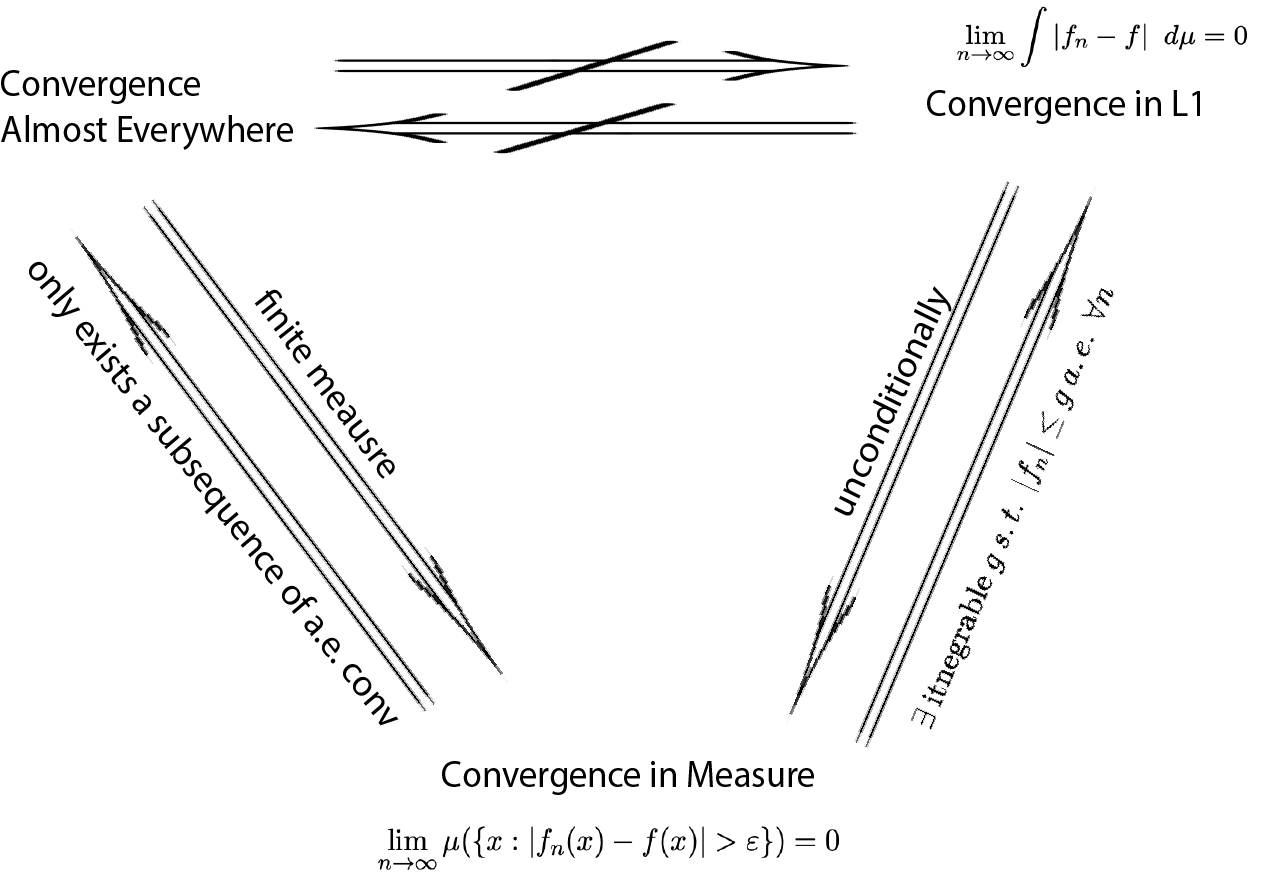
\includegraphics[width=0.7\linewidth]{mode_of_convergence.png}
	\end{figure}
	
	\begin{proposition}[Dominated Convergence Theorem II]
		Suppose $f_n \overset{\mu}{\to} f$, and $\exists$ integrable $g$ such that $\abs{f_n} \leq g$ a.e. for all $n$. Then, $f_n \overset{L^1}{\to} f$, in particular, $\int f_n\ d\mu \to \int f\ d\mu$.
		\begin{proof}
			Suppose, for contradiction, $f_n \centernot \to f$ in $L^1$. Equivalently, there exists $\varepsilon$ and a subsequence $f_{n_k}$ such that for all $k$:
			\begin{align}
				\int \abs{f_{n_k} - f}\ d\mu \geq \varepsilon \quad (\dagger)
			\end{align}
			But the convergence in measure implies $f_{n_k} \to f$ in measure as well. Then there exists a subsequence $n_{k_\ell}$ such that $f_{n_{k_\ell}} \to f$ almost everywhere.
			
			By the previous dominated convergence theorem, $\lim_{\ell \to \infty} \int \abs{f_{n_{k_\ell}} - f}\ d\mu = 0$, contradicts $(\dagger)$.
		\end{proof}
	\end{proposition}
	
	\section{Normed Space}
	\begin{definition}
		Let $V$ be a vector space over $\R$ (over $\C$), a \textbf{norm} on $V$ is a function $\norm{\cdot}: V \to \R$ such that
		\begin{enumerate}
			\item $\norm{x} \geq 0\ \forall x \in V$,
			\item $\norm{x} = 0 \iff x = 0$,
			\item $\norm{a x} = \abs{a} \norm{x}$ for all $a \in \R(\in \C)$,
			\item (Triangle Inequality) $\norm{x + y} \leq \norm{x} + \norm{y}\ \forall x, y \in V$.
		\end{enumerate}
	\end{definition}
	
	\begin{example}
		For $V = \R^n$, \ul{for every $p \geq 1$}, the $L^p$ norm is defined as
		\begin{align}
			\norm{x}_{L^p} = \left( \sum_{i=1}^n \abs{x_i}^p \right)^{1/p}
		\end{align}
		\emph{Note: for $p < 1$, the triangle inequality fails.}
	\end{example}
	
	\begin{example}
		Let $C[a, b]$ denote the collection of continuous functions from $[a, b]$ to $\R$, where $[a, b]$ is a compact interval.
		
		The sup norm is defined as
		\begin{align}
			\norm{f}_\infty = \sup_{x \in [a, b]} \abs{f(x)}
		\end{align}
		The 1-norm is defined as
		\begin{align}
			\norm{f}_1 = \int_{[a, b]} \abs{f}\ d\lambda
		\end{align}
	\end{example}
	
	\begin{definition}
		Let $S$ be a set, a \textbf{metric} $d$ on $S$ is a function $d: S \times S \to \R$ such that for all $x, y, z \in S$:
		\begin{enumerate}
			\item $d(x, y) \geq 0$,
			\item $d(x, y) = 0 \iff x = y$,
			\item $d(x, y) = d(y, x)$,
			\item $d(x, y) \leq d(x, z) + d(y, z)$.
		\end{enumerate}
	\end{definition}
	
	\begin{proposition}
		A norm induces a metric: $d(x, y) := \norm{x - y}$.
		
		\emph{Note: the converse is false, i.e., there are metrics not induced by any norm. For example, $d(x, y) := \id{x = y}$ is in general not induced by any norm.}
	\end{proposition}
	
	\begin{definition}
		Let $S$ be a set with a metric $d$, a sequence of points $x_n$ converges to $x \in S$ if
		\begin{align}
			\lim_{n \to \infty} d(x_n, x) = 0
		\end{align}
		A sequence is \textbf{Cauchy} with respect to $d$ if $\forall \varepsilon > 0, \exists n_0 \in \N\ s.t.\ \forall m, n \geq n_0, d(x_m, x_n) < \varepsilon$.
	\end{definition}
	
	\begin{definition}
		A metric space w.r.t $d$ is \textbf{complete} if every Cauchy sequence w.r.t. $d$ converges to somewhere in the space.
	\end{definition}
	
	\begin{example}
		$C[a, b]$ with the supremum norm is complete.
	\end{example}
	
	\begin{example}
		$C[a, b]$ with $L^1$ norm is not complete.
		\begin{proof}
			Using counter-example: for $[a, b] = [-1, 1]$,
			\begin{align}
				f_n(x) = \begin{cases}
					0 &\tx{ if } x \in [-1, 0] \\
					nx & \tx{ if } x \in(0, 1/n) \\
					1 &\tx{ if } x \in [1/n, 1] \\
				\end{cases}
			\end{align}
			The sequence of $f_n$ is Cauchy but converges to $f = \id{x \geq 0} \notin C[a,b]$.
		\end{proof}
	\end{example}
	
	\begin{proposition}
		$C[a, b]$ under sup-norm is complete.
		\begin{proof}
			Suppose $f_n$ is a Cauchy sequence in $C[a, b]$ under supremum norm. For all $x \in [a, b]$,
			\begin{align}
				f_n(x) - f_m(x) \leq \norm{f_n - f_m}_\infty \to 0
			\end{align}
			since $f_n$ is Cauchy. Therefore, $f_n(x)$ is a Cauchy sequence in $\R$ and $\lim_{n\to\infty} f_n(x)$ exists. Define $f$ to be the point-wise limit of $f_n$.
			
			Claim: $f \in C[a, b]$ and $f_n \to f$ in sup-norm.
			
			For all $\varepsilon > 0$, there exists $N$, such that for all $m, n \geq N$,
			\begin{align}
				\norm{f_m - f_n}_\infty < \varepsilon
			\end{align}
			Therefore, for all $x \in [a, b]$, $\abs{f_n(x) - f_m(x)} < \norm{f_m - f_n}_\infty < \varepsilon$.
			
			Fixing $n$, take $m \to \infty$, this shows for all $n \geq N$, for all $x \in [a, b]$
			\begin{align}
				\abs{f(x) - f_n(x)} = \lim_{m\to\infty} \abs{f_m(x) - f_n(x)} \leq \varepsilon
			\end{align}
			Therefore, for all $n \geq N$, $\norm{f - f_n}_\infty \leq \varepsilon$. Hence $f \to f_n$ in sup-norm.
			
			Now show the continuity of $f$: take $x_0 \in [a, b]$, given $\varepsilon > 0$, since $f_n \to f$ in sup-norm, there exists $N$ such that for all $n \geq N$,
			\begin{align}
				\norm{f - f_n}_\infty \leq \frac{\varepsilon}{3}
			\end{align}
			In particular, $\norm{f - f_N}_\infty \leq \frac{\varepsilon}{3}$.
			
			Moreover, since $f_N$ is continuous, $\exists \delta > 0$ such that $\abs{x - x_0} < \delta \implies \abs{f_N(x) - f_N(x)} < \varepsilon / 3$ for every $x$. Take any $x \in \mc{B}_\delta(x_0)$, by triangle inequality,
			\begin{align}
				\abs{f(x) - f(x_0)} &\leq \abs{f(x) - f_N(x)} + \abs{f_N(x) - f_N(x_0)} + \abs{f_N(x_0) - f(x_0)} \\
				&\leq \frac{\varepsilon}{3} + \frac{\varepsilon}{3} + \frac{\varepsilon}{3} = \varepsilon
			\end{align}
			Hence, $f \in C[a, b]$. 
		\end{proof}
	\end{proposition}
	
	\section{Functional Analysis: $L^p$ Spaces}
	\emph{We will firstly define $\mc{L}^p$ spaces, which is a little simpler than $L^p$ spaces.}
	\begin{definition}
		Let $(X, \mc{A}, \mu)$ be a measure space, for every $1 \leq p < \infty$, the $\mc{L}^p(X, \mc{A}, \mu, \R)$ space is the collection of all measurable functions $f: X \to \R$ such that
		\begin{align}
			\int \abs{f}^p\ d\mu < \infty
		\end{align}
		Similarly, $\mc{L}^p(X, \mc{A}, \mu, \C)$ denotes the collection of all measurable functions $f: X \to \C$ such that $\int \abs{f}^p\ d\mu < \infty$.
	\end{definition}
	\emph{Thought out this notes, we use $\mc{L}^p$ to denote $\mc{L}^p(X, \mc{A}, \mu, \R)$ or $\mc{L}^p(X, \mc{A}, \mu, \C)$.}
	\begin{proposition}[$\mc{L}^p$ space is a vector space]
		Note that $0 \in \mc{L}^p$, and if $f \in \mc{L}^p$ and $\alpha \in \R/\C$, then
		\begin{align}
			\int \abs{\alpha f}^p\ d\mu = \abs{\alpha}^p \int \abs{f}^p\ d\mu < \infty
		\end{align}
		Therefore, $\alpha f \in \mc{L}^p$.
		
		For all $x \in X$,
		\begin{align}
			\abs{f(x) + g(x)}^p &\leq (\abs{f(x)} + \abs{g(x)})^p \\
			&\leq (2 \max\{\abs{f(x)}, \abs{g(x)}\})^2 \\
			&\leq 2^p \max\{\abs{f(x)}^p, \abs{g(x)}^p\} \\
			&\leq 2^p (\abs{f(x)}^p + \abs{g(x)}^p) \\
			\implies \int \abs{f+g}^p\ d\mu &< \infty \\
			\implies f + g &\in \mc{L}^p
		\end{align}
		Hence, $\mc{L}^p$ is a vector space.
	\end{proposition}
	
	\begin{definition}
		Let $\mc{L}^\infty(X, \mc{A}, \mu, \R/\C)$ be the set of all \ul{bounded} measurable $f: X \to \R/\C$.
	\end{definition}
	
	\begin{definition}
		For $f \in \mc{L}^p$ with $p < \infty$, define
		\begin{align}
			\norm{f}_p = \left(\int \abs{f}^p\ d\mu \right)^{\frac{1}{p}}
		\end{align}
		for $p = \infty$, $\norm{f}_\infty$'s definition is a little bit more complicated, for continuous functions, it collides with the sup-norm. However, it's not the same as sup-norm for discontinuous functions.
	\end{definition}
	
	\begin{definition}
		Given a measure space $(X, \mc{A}, \mu)$, a set $B$ is called \textbf{$\mu$-null/negligible} if $B \subseteq A$ for some $A \in \mc{A}$ with $\mu(A) = 0$.
		
		A subset $N \subseteq X$ is called \textbf{locally $\mu$-null} if $\forall A \in \mc{A}$ with $\mu(A) < \infty$, $A \cap N$ is $\mu$-null.
		
		A property of elements of $X$ is said to hold \textbf{locally a.e.} if the set on which it fails is locally $\mu$-null.
	\end{definition}
	\emph{We use this notion of locally null to circumvent non-sigma finite cases.}
	
	\begin{definition}
		For $f \in \mc{L}^\infty$, define
		\begin{align}
			\norm{f}_\infty = \inf \left\{
			M \geq 0 : \tx{the set of all $x$ with $\abs{f(x)} > M$ is locally $\mu$-null.}
			\right\}
		\end{align}
		this is called the \textbf{essential supremum} of $\abs{f}$. Equivalently, $\norm{f}_\infty$ is the infimum of $M$ such that $\abs{f(x)} \leq M$ locally a.e.
		
		Note that $\norm{f}_\infty$ is only a semi-norm, we may modify a function on a measure-zero set without changing the value of $\norm{f}_\infty$.
		
		Our previous definitions of semi-norms on $\mc{L}^p$ spaces satisfy
		\begin{align}
			\norm{f}_p = 0 \iff \int \abs{f}^p\ d\mu = 0 \iff \abs{f}^p = 0\ a.e. \iff f = 0\ a.e.
		\end{align}
		This definition of semi-norm on $\mc{L}^\infty$ ensures $\norm{f}_\infty = 0 \iff f = 0\ a.e.$.
	\end{definition}
	
	\begin{example}
		Take $X = [0, 1]$ and $\mu = \lambda$,
		\begin{align}
			f(x) = \begin{cases}
				x &\tx{ if } x \neq \frac{1}{2} \\
				2 &\tx{ otherwise}
			\end{cases}
		\end{align}
		Then $\norm{f}_\infty=1$ but $\sup f = 2$. To see this, note that $\{x : \abs{f(x)} > 1\} = \{1/2\}$ has zero measure. However, for any $M < 1$, the same has non-zero Lebesgue measure.
	\end{example}
	
	\begin{proposition}
		\begin{align}
			&\mu\left(\{
			x : \abs{f(x)} > \norm{f}_\infty
			\}\right) \tx{ is locally $\mu$-null.} \\
			&\mu\left(\{
			x : \abs{f(x)} > c
			\}\right) \tx{ is not locally $\mu$-null } \forall c < \norm{f}_\infty
		\end{align}
	\end{proposition}
	
	\begin{lemma}
		Countable union of locally $\mu$-null sets is locally $\mu$-null.
	\end{lemma}
	
	\begin{proposition}
		$\norm{f}_p$ and $\norm{f}_\infty$ are semi-norms.
	\end{proposition}
	
	\begin{definition}
		Given $p \in (1, \infty)$, the \textbf{conjugate exponent} $q$ is defined as
		\begin{align}
			\frac{1}{p} + \frac{1}{q} = 1
		\end{align}
		That is,
		\begin{align}
			q = \frac{p}{p-1}
		\end{align}
		For $p = \infty$, $q=1$.
	\end{definition}
	
	\begin{lemma}[Young's Inequality]
		Take $p \in (1, \infty)$, let $q$ be the conjugate exponent of $p$, then for all $x, y \geq 0$,
		\begin{align}
			x y \leq \frac{x^p}{p} + \frac{y^q}{q}
		\end{align}
		\begin{proof}
			
		\end{proof}
	\end{lemma}
	
	\begin{theorem}[H\"older's Inequality]
		Let $(X, \mc{A}, \mu)$ be a measure space, take $1 \leq p \leq \infty$, and $q$ be it's conjugate exponent. Take $f \in \mc{L}^p$, $g \in \mc{L}^q$, then
		\begin{align}
			fg \in \mc{L}^1
		\end{align}
		and
		\begin{align}
			\norm{fg}_1 \leq \norm{f}_p \norm{g}_q
		\end{align}
	\end{theorem}
	
	\begin{example}
		Take $X = \{x_1,\cdots, x_n\}$ and $\mu$ to be the counting measure on $X$. Let $p = q = 2$ and $f, g \in \mc{L}^2$. Define $v = (f(x_1), \dots, f(x_n)) \in \R^n$ and $u = (g(x_1),\dots,g(x_n)) \in \R^n$.
		\begin{align}
			\norm{fg}_1 = \sum_{i=1}^n \mu(\{x_i\}) \abs{f(x_i) g(x_i)} = \sum_{i=1}^n \abs{f(x_i) g(x_i)}
		\end{align}
		Therefore,
		\begin{align}
			\abs{\inner{v}{u}} = \abs{\sum_{i=1}^n f(x_i) g(x_i)} \leq \norm{fg}_1
		\end{align}
		In this finite dimensional case with counting measure,
		\begin{align}
			\norm{f}_2 = \sqrt{\sum_{i=1}^n \mu(\{x_i\}) f(x_i)^2} = \sqrt{\sum_{i=1}^n f(x_i)^2} = \norm{v}_2
		\end{align}
		The same holds for $g$, in this case H\"older's inequality reduces to cauchy-Switchz inequality.
	\end{example}
	
	\begin{proof}
		
	\end{proof}
	
	\begin{theorem}[Minkowski's Inequality]
		Let $(X, \mc{A}, \mu)$ be a measure space. Take $1 \leq p \leq \infty$. If $f, g \in \mc{L}^p(X, \mc{A}, \mu)$, then $f + g \in \mc{L}^p$ and $\norm{f+g}_p \leq \norm{f}_p + \norm{g}_p$.
		\begin{proof}
			First, suppose that $p \in (1, \infty)$. Let $q$ be the conjugate exponent of $p$. We have already shown that $\mc{L}^p$ is a vector space, so $f + g \in \mc{L}^p$.
			
			Note that
			\begin{align}
				1/p + 1/q = 1 \implies (p+q)/(pq) = 1 \implies p + q = pq \implies p = (p-1)q
			\end{align}
			Therefore,
			\begin{align}
				\int (\abs{f+g}^{p-1})^q\dmu = \int \abs{f+g}^p\dmu < \infty
			\end{align}
			Therefore, $\abs{f+g}^{p-1} \in \mc{L}^q$. By H\"older's inequality,
			\begin{align}
				\int \abs{f+g}^p\dmu &= \int \abs{f+g} \abs{f+g}^{p-1}\dmu \\
				&\leq \int \abs{f}\abs{f+g}^{p-1}\dmu + \int \abs{g}\abs{f+g}^{p-1}\dmu \\
				&\leq \norm{f}_p \norm{\abs{f+g}^{p-1}}_q  + \norm{g}_p \norm{\abs{f+g}^{p-1}}_q
			\end{align}
			where
			\begin{align}
				\norm{\abs{f+g}^{p-1}}_q &= \left(\int (\abs{f+g}^{p-1})^q \right)^{1/q} = \left(\int \abs{f+g}^p \right)^{1/q}
			\end{align}
			If $\norm{f+g}_p = 0$, we are done. Suppose not, divide $(\int \abs{f+g}^p\dmu)^{1/q}$ on both sides,
			\begin{align}
				\frac{\int \abs{f+g}^p\dmu}{(\int \abs{f+g}^p\dmu)^{1/q}} &\leq \norm{f}_p + \norm{g}_p \\
				\implies (\int \abs{f+g}^p\dmu)^{1-1/q} &= (\int \abs{f+g}^p\dmu)^{1/p} = \norm{f+g}_p \leq \norm{f}_p + \norm{g}_p 
			\end{align}
			When $p = 1$,
			\begin{align}
				\norm{f+g}_1 = \int \abs{f+g}\dmu \leq \int (\abs{f}+\abs{g})\dmu = \norm{f}_1 + \norm{g}_1
			\end{align}
			When $p = \infty$, define
			\begin{align}
				N_1 = \{x: \abs{f(x)} > \norm{f}_\infty\} \\
				N_2 = \{x: \abs{g(x)} > \norm{g}_\infty\}
			\end{align}
			Then $N_1$ and $N_2$ are locally $\mu$-null, so is $N_1 \cup N_2$. For $x \notin N_1 \cup N_2$,
			\begin{align}
				\abs{f(x) + g(x)} \leq \abs{f(x)} + \abs{g(x)} \leq \norm{f}_\infty + \norm{g}_\infty
			\end{align}
		\end{proof}
	\end{theorem}
	\emph{Note that $\norm{\cdot}_p$ is a \textbf{semi-norm} on $\mc{L}^p$, to make it a norm, we introduce the $L^p$ space.}
	\begin{definition}
		For $1 \leq p < \infty$, define the class of zero vectors
		\begin{align}
			\mc{N}^p := \{f \in \mc{L}^p : f \tx{ is measurable and } f = 0\ a.e.\}
		\end{align}
		which is a subspace of $\mc{L}^p$. Define $L^p$ to be the quotient space:
		\begin{align}
			L^p(X, \mc{A}, \mu) := \mc{L}^p(X, \mc{A}, \mu) / \mc{N}^p(X, \mc{A}, \mu)
		\end{align}
		That is, an element $[f] \in L^p$ (an equivalent class) is the collection of all $g \in \mc{L}^p$ such that $f - g = 0$ almost everywhere:
		\begin{align}
			L^p \ni [f] := \{g \in \mc{L}^p : f - g \in \mc{N}^p\}
		\end{align}
		Then $L^p$ is a vector space over $\R$ or $\C$, and $\norm{\cdot}_p$ is well-defined: for any $f$, for all $g \in [f]$, $\norm{f}_p = \norm{g}_p$ since $f = g$ almost everywhere so their integrals are the same. Most importantly, $\norm{\cdot}_p$ is a norm on $L^p$.
		
		For $p = \infty$, we define
		\begin{align}
			\mc{N}^\infty := \{f : f \tx{ is bounded, measure and } f = 0\ a.e.\}
		\end{align}
		Then $L^\infty := \mc{L}^p / \mc{N}^p$.
	\end{definition}
	\emph{Note that $L^p$ for $1 \leq p \leq \infty$ is also a vector space with equivalence relations. In general, we treat $L^p$ as a space of functions instead of a space of classes of functions.}
	\begin{proposition}
		Convergence in $L^p$ ($1 \leq p < \infty$) implies convergence in measure.
		\begin{proof}
			By Markov's inequality,
			\begin{align}
				\mu(\{x : \abs{f_n(x) - f(x)} > \varepsilon \}) &= \mu(\{x : \abs{f_n(x) - f(x)}^p > \varepsilon^p \}) \\
				&\leq \frac{\int \abs{f_n - f}^p\dmu}{\varepsilon^p} \to 0 \tx{ as } n \to \infty
			\end{align}
		\end{proof}
	\end{proposition}
	
	\begin{corollary}
		Let $f_n \to f$ in $L^p$ with $1 \leq p < \infty$, then there exists a subsequence $f_{n_k} \to f$ a.e.
		\begin{proof}
			As convergence in $L^p$ implies convergence in measure, which further implies existence of a.e. converging subsequences.
		\end{proof}
	\end{corollary}
	
	\begin{theorem}
		For any $1 \leq p \leq \infty$, the $\norm{\cdot}_p$ norm on $L^p$ is complete.
		\begin{proof}
			For $1 \leq p < \infty$, let $(f_n)$ be a Cauchy sequence in $L^p$.
			
			\emph{Step 1: Find a subsequence $(f_{n_k})$ such that $\norm{f_{n_k} - f_{n_{k+1}}}_p \leq 2^{-k}$ for all $k$.} By Cauchy property, we may find $n_1$ such that $\norm{f_{n_1} - f_n} \leq 2^{-1}$ for all $n \geq n_1$. Also, find a $n_2 \geq n_1$ such that $\norm{f_{n_2} - f_n} \leq 2^{-2}$ for all $n \geq n_2$, etc.
			
			\emph{Step 2: construct the limit} Define
			\begin{align}
				A_k := \{x: |f_{n_k}(x) - f_{n_{k+1}}(x)| > 2^{-k/2}\}
			\end{align}
			Then, by Markov's inequality,
			\begin{align}
				\mu(A_k) &\leq \frac{\int |f_{n_k} - f_{n_{k+1}}|^p \dmu}{(2^{-k/2})^p} \\
				&\leq \frac{2^{-kp}}{(2^{-k/2})^p} = 2^{-kp/2}
			\end{align}
			Thus, $\sum_{k=1}^\infty \mu(A_k) < \infty$. Define
			\begin{align}
				B := \{x : x \in \tx{ infinitely many} A_k\} = \bigcap_{k=1}^\infty \bigcup_{j=k}^\infty A_j
			\end{align}
			By Borel-Cantelli lemma, $\mu(B) = 0$. Take any $x \notin B$, then for sufficiently large $k$,
			\begin{align}
				\abs{f_{n_k}(x) - f_{n_{k+1}}} \leq 2^{-k/2}
			\end{align}
			This shows for all $x \notin B$, the constructed $(f_{n_k}(x))$ is a Cauchy sequence in $\R$, therefore, it's convergent.
			
			Define the almost point-wise limit
			\begin{align}
				f(x) := \begin{cases}
					\lim_{k \to \infty} f_{n_k}(x) &\tx{ if } x \notin B \\
					0 &\tx{ if } x \in B
				\end{cases}
			\end{align}
			\emph{Step 3: Show $f_n \to f$ in $L^p$.} Note that $f_{n_k} \to f$ almost everywhere, so that $|f|^p \to |f_{n_k}|^p$. By Fatou's lemma,
			\begin{align}
				\int \abs{f}^p\dmu \leq \liminf_{k\to\infty} \int \abs{f_{n_k}}^p\dmu
			\end{align}
			But the Cauchy property of $f_n$ implies that $\sup_n \norm{f_n}_p < \infty$ (find $n$ such that $\norm{f_n - f_m}_p \leq 1$ for all $m \geq n$. Thus, $\forall m \geq n$, $\norm{f_m}_p \leq \norm{f_n - f_m}_p + \norm{f_n}_p \leq 1 + \norm{f_n}_p$.
			Therefore, $\norm{f}_p < \infty$.
			
			For any $\varepsilon > 0$, we can find $N$ so large that $\norm{f_n - f_m}_p < \varepsilon$ for all $n, m \geq N$ since $f_n$ is Cauchy.
			By Fatou's lemma, for all $n \geq N$,
			\begin{align}
				\int \abs{f_n - f}^p\dmu \leq \liminf_{n \to \infty} \int \abs{f_n - f}^p\dmu
			\end{align}
			But when $k$ is so large that $n_K \geq N$, we have
			\begin{align}
				\int \abs{f_n - f_{n_k}}^p\dmu = \norm{f_n - f_{n_k}}_p^p \leq \varepsilon^p
			\end{align}
			Thus, fo all $n \geq N$, $\norm{f - f_n}_p \leq \varepsilon$.
		\end{proof}
		\begin{proof}[Proof. for $p = \infty$ case]
			Let $f_n$ be Cauchy in $L^\infty$, as before, find a subsequence $f_{n_k}$ such that
			\begin{align}
				\norm{f_{n_k} - f_{n_{k+1}}}_\infty \leq 2^{-k}\quad \forall k
			\end{align}
			Then for all $k$, there exists a locally $\mu$-null set $N_k$ such that for all $x \notin N_k$.
			\begin{align}
				\abs{f_{n_k}(x) - f_{n_{k+1}}(x)} \leq 2^{-k}
			\end{align}
			Let $N = \bigcup_{k=1}^\infty N_k$, so that $N$ is locally $\mu$-null as well.
			Then for all $x \notin N$, $f_{n_k}(x)$ is a Cauchy sequence of real numbers, define $f(x) = \lim_k f_{n_k}(x)$ outside $N$ and $f(x) = 0$ on $N$.
			
			Claim: $f_n \to f$ in $L^\infty$. Note that for all $x \notin N$, for all $k$,
			\begin{align}
				\abs{f(x) - f_{n_k}(x)} \leq \sum_{j=k}^\infty \abs{f_{n_j}(x) - f_{n_{j+1}}(x)} \leq \sum_{j=k}^\infty 2^{-j} = 2^{-k+1}
			\end{align}
			Thus, $\norm{f - f_{n_k}}_\infty \leq 2^{-k+1}$.
			
			Take any $\varepsilon > 0$, find $N$ so large that $\forall m, n \geq N$, $\norm{f_m - f_n}_\infty \leq \varepsilon$. Then find $k$ so large that $n_k \geq N$ and $2^{-k+1} \leq \varepsilon$. Then for all $n \geq N$,
			\begin{align}
				\norm{f - f_n}_\infty \leq \norm{f - f_{n_k}}_\infty + + \norm{f_{n_k} - f_n} \leq 2 \varepsilon
			\end{align}
			Taking $\varepsilon' = \varepsilon/2$ concludes $f_n \to f$ in $L^\infty$.
		\end{proof}
	\end{theorem}
	
	\section{Signed and Complex Measures}
	\begin{definition}
		Let $(X, \mc{A})$ be a measurable space, let $\mu: \mc{A} \to [-\infty, \infty]$ be a function. We say that $\mu$ is a \textbf{signed measure} if
		\begin{enumerate}
			\item $\mu(\varnothing) = 0$,
			\item and $\mu$ is countable additive: for all disjoint $A_1, A_2, \dots \in \mc{A}$, $\mu(\cup_{i=1}^\infty A_i) = \sum_{i=1}^\infty \mu(A_i)$.
		\end{enumerate}
	\end{definition}
	\emph{From now on, we use \textbf{measure} to denote the conventional notion of measure, that is, $\mu: \mc{A} \to [0, \infty]$ with $\mu(\varnothing) = 0$ and countable additivity. The term \textbf{signed measure} denotes functions $\mu: \mc{A} \to [-\infty, \infty]$ with above properties.}
	\begin{remark}
		Note that the countable additivity does not change if we permute $A_i$'s, thus, implies $\sum_{i=1}^\infty \mu(A_i)$ should now change under any rearrangement of the terms. This implies that if $\mu(\cup_{i=1}^\infty A_i)$ is finite, $\sum_{i=1}^\infty |\mu(A_i)| < \infty$.
	\end{remark}
	
	\begin{proposition}
		If $\mu$ is a signed measure, then $\mu$ cannot be both $\infty$ and $-\infty$.
		\begin{proof}
			\textbf{Case 1}: if $\mu(X) \in \R$, then for any $A$, $\mu(X) = \mu(A) + \mu(A^c)$, both of $\mu(A)$ and $\mu(A^c)$ must be finite. 
			
			\textbf{Case 2}: if $\mu(X) = \infty$, then $\mu(A) + \mu(A^c) = \mu(X) = \infty$, none of $\mu(A)$ or $\mu(A^c)$ can be $-\infty$.
			
			\textbf{Case 3}: if $\mu(X) = - \infty$, then $\mu(A) + \mu(A^c) = \mu(X) = - \infty$, none of $\mu(A)$ or $\mu(A^c)$ can be $\infty$. 
		\end{proof}
	\end{proposition}
	
	\begin{proposition}
		If $\mu(A)$ is finite (i.e., in $\R$), then $\mu(B) \in \R$ for any $B \subseteq A$, $B \in \mc{A}$.
		\begin{proof}
			$\mu(A) = \mu(B) + \mu(A \backslash B) \in \R$, both $\mu(B)$ and $\mu(A \backslash B)$ must be finite.
		\end{proof}
	\end{proposition}

	\begin{definition}
		A signed measure is called \textbf{finite} if $\mu(A) \in \R$ for all $A \in \mc{A}$.
	\end{definition}
	
	\subsection{Construction of Signed Measures}

	\begin{example}[Relationship between integrable function and measure]
		Let $(X, \mc{A}, \mu)$ be a measure space, let $f \in L^1$, define $\nu(A) = \int_A f\dmu$, then $\nu$ is a signed measure.
	\end{example}

	\begin{example}[Construction of signed measure]
		If $\nu_1$ and $\nu_2$ are measures and a least one of them if finite, then $\nu_1 - \nu_2$ is a signed measure.
	\end{example}
	
	\subsection{Hahn Decomposition Theorem}
	\par Let $(X, \mc{A})$ be a measurable space and let $\mu$ be a signed measure on $(X, \mc{A})$.
	\begin{definition}
		A set $A \in \mc{A}$ is called a \textbf{positive set for $\mu$} if $\mu(B) \geq 0$ for all $B \subseteq A, B \in \mc{A}$.
		Similarly, a set $A \in \mc{A}$ is called a \textbf{negative set for $\mu$} if $\mu(B) \leq 0$ for all $B \subseteq A, B \in \mc{A}$.
	\end{definition}
	
	\begin{lemma}
		If $A \in \mc{A}$ satisfies $- \infty < \mu(A) < 0$, then there exists a negative set $B \subseteq A$ such that $\mu(B) \leq \mu(A) (<0)$.
		\begin{proof}
			Let $\delta_1 = \sup\{\mu(E) : E \in \mc{A}, E \subseteq A\}$, note that $\delta_1 \geq 0$ since $\mu(\varnothing) = 0$.
			
			By the definition of $\delta_1$ we can find $A_1 \subseteq A$ such that $\mu(A_1) \geq \delta_1 / 2$ if $\delta_1 < \infty$, or $\mu(A_1) \geq 1$ if $\delta_1 = \infty$. Thus, $\mu(A_1) \geq \min\{\delta_1/2, 1\}$.
			
			Let $\delta_2 = \sup\{\mu(E) : E \in \mc{A}, E \subseteq A \backslash A_1 \}$, similarly, we can choose $A_2 \subseteq A \backslash A_1$ and $A_2 \in \mc{A}$ such that $\mu(A_2) \geq \min\{\delta_2/2, 1\}$.
			
			Similarly, choose $A_n \in \mc{A}$, $A_n \subseteq A \backslash (A_1 \cup \dots A_{n-1})$, such that $\mu(A_n) \geq \min\{\delta_n/2, 1\}$.
			Then by definition, $A_1, A_2, \dots$ are disjoint, they are all contained in $A$.
			
			Let $B = A \backslash (\bigcup_{i=1}^\infty A_i)$.
			
			Claim: this $B$ is a negative set such that $\mu(B) \leq \mu(A)$.
			\begin{tcolorbox}
				Note that $\mu(A) \in \R \implies \mu(B) \in \R$. Thus, $\mu(\bigcup_{i=1}^\infty A_i) = \mu(A) - \mu(B) \in \R$.
				
				But $\mu(\bigcup_{i=1}^\infty A_i) = \sum_{i=1}^\infty \mu(A_i)$ since $A_n's$ are disjoint. Therefore, $\mu(A_i) \to 0$ as $i \to \infty$.
				However, $\mu(A_i) \geq \min\{\delta_i/2, 1\} \geq 0$.
				It must be $\delta_i \to 0$ as $i \to 0$.
				
				Take any $E \subseteq B$ such that $E \in \mc{A}$. Then $E \subseteq B \subseteq A \backslash (A_1 \cup \dots A_{n-1})$ for all $n \in \N$. So by definition of $\delta_n$, we have $\mu(E) \leq \delta_n$, thus $\mu(E) \leq 0$ as we take $n \to \infty$. Hence $B$ is a negative set.
				
				Finally, since $\mu(A_i) \to 0$, $\mu(B) = \mu(A) - \sum_{i=1}^\infty \mu(A_i) \leq \mu(A)$.
			\end{tcolorbox}
		\end{proof}
	\end{lemma}
	
	\begin{theorem}[Hahn Decomposition Theorem]
		Let $(X, \mc{A})$ be a measurable space and $\mu$ a \ul{signed measure} on $(X, \mc{A})$. Then, there exists \ul{disjoint} $P \cup N$ in $\mc{A}$ such that $X = P \cup N$ such that $P$ is a positive set for $\mu$ and $N$ is a negative set for $\mu$.
		\begin{proof}
			Since $\mu$ is a signed measure, we know that it cannot take value at both $\infty$ and $-\infty$. WLOG, suppose $\mu$ never takes value $-\infty$.
			Let
			\begin{align}
				L = \inf\{\mu(A) : A \in \mc{A}\ s.t.\ A \tx{ is negative}\}
			\end{align}
			Then there exists a sequence of negative sets $A_n$ such that $\mu(A_n) \to L$. Define $B = \cup_{n=1}^\infty A_n$. For sure, $B \in \mc{A}$.
			\begin{tcolorbox}
				\textbf{Claim}: $B$ is a negative set.
				
				Take and $E \subseteq B$ such that $E \in \mc{A}$, then
				\begin{align}
					E = E \cap B = \bigcup_{i=1}^\infty E \cap A_i = \bigcup_{i=1}^\infty E \cap (A_i \backslash (A_1 \cup \dots \cup A_{i-1}))
				\end{align}
				where the last step holds because we only consider the net incremental at each step. Moreover, $\{E \cap (A_i \backslash (A_1 \cup \dots \cup A_{i-1}))\}_i$ are disjoint.
				
				Thus, 
				\begin{align}
					\mu(E) = \sum_{i=1}^\infty \mu(\underbrace{E \cap (A_i \backslash (A_1 \cup \dots \cup A_{i-1}))}_{\subseteq A_i})
				\end{align}
				Since $A_i$'s are all negative sets, we must have $\mu(E) \leq 0$ and $B$ is a negative set.
			\end{tcolorbox}
			\begin{tcolorbox}
				\textbf{Claim}: $\mu(B) = L$.
				
				Since $A_n \subseteq B$,
				\begin{align}
					\mu(B) = \mu(A_n) + \mu(B \backslash A_n)
				\end{align}
				But $B$ is a negative set, so $\mu(B \backslash A_n)\leq 0$. Thus,
				\begin{align}
					\mu(B) \leq \mu(A_n)\quad \forall n \in \N
				\end{align}
				Thus, $\mu(B) \leq \lim_n \mu(A_n) = L$. But $B$ itself is a negative set, and $L$ is the infimum, so $L \leq \mu(B)$.
			\end{tcolorbox}
			In particular, we've shown that $L > -\infty$ since $\mu$ never takes value at $-\infty$.
			
			Let $N = B$ and $P = N^c$. Since $B \in \mc{A}$, both $N, P \in \mc{A}$.
			\begin{tcolorbox}
				Claim: $P$ is a positive set.
				
				Suppose not, then $\exists A \subseteq P$ such that $A \in \mc{A}$ and $-\infty < \mu(A) < 0$.
				
				By the lemma, there exists a negative set $D \subseteq A$ and $\mu(D) \leq \mu(A) < 0$. Note that $D \subseteq A \subseteq P$, but then $N \cup D$ is a negative set as a union of negative sets.
				Then,
				\begin{align}
					\mu(N \cup D) = \mu(N) + \mu(D)
					= L + \mu(D) < L
				\end{align}
				which leads to a contradiction.
			\end{tcolorbox}
			Consequently, this $X = N \cup P$ is a Hahn decomposition.
		\end{proof}
	\end{theorem}
	
	\begin{theorem}[Jordan Decomposition Theorem]
		Every signed measure is the difference of two measures, at least one of which is finite.
		\begin{align}
			\mu = \mu^+ - \mu^-
		\end{align}
		\begin{proof}
			Let $\mu$ be a signed measure, let $(N, P)$ be a Hahn decomposition of $X$.
			
			For every $A \in \mc{A}$, define
			\begin{align}
				\mu^+(A) &= \mu(A \cap P) \\
				\mu^-(A) &= - \mu(A \cap N)
			\end{align}
			Since $P$ is a positive set, $\mu^+(A) \geq 0$, similarly, since $N$ is negative, $\mu^-(A) \geq 0$ as well.
			
			Let $A_1, A_2, \dots$ be disjoint sets in $\mc{A}$, then
			\begin{align}
				\mu^+(\cup_i A_i) &= \mu(P \cap (\cup_i A_i)) \\
				&= \mu(\cup_i (P \cap A_i)) \\
				&= \sum_i \mu(P \cap A_i) \\
				&= \sum_i \mu^+(A_i)
			\end{align}
			So $\mu^+$ is a measure. Similarly, $\mu^-$ is a measure as well.
			\begin{align}
				\mu^+(A) - \mu^-(A) = \mu(A \cap P) + \mu(A \cap N) = \mu(A)
			\end{align}
			Therefore, $\mu = \mu^+ - \mu^-$. Lastly, note that $\mu(X) = \mu(P) + \mu(N) = \mu^+(P) - \mu^-(N)$, we need at least one of them to be finish in order to avoid subtracting infinity from infinity.
		\end{proof}
	\end{theorem}
	
	\begin{proposition}
		Let $(\mu^+, \mu^-)$ be the decomposition of a signed measure from Hahn decomposition $(P, N)$, that is, $\mu^+(A) = \mu(A \cap P)$ and $\mu^-(A) = - \mu(A \cap N)$ for any $A \in \mc{A}$. Then,
		\begin{align}
			\mu^+(A) &= \sup\{\mu(B) : B \subseteq A, B \in \mc{A}\} \\
			\mu^-(A) &= \sup\{-\mu(B) : B \subseteq A, B \in \mc{A}\}
		\end{align}
		\begin{proof}
			Take any $A \in \mc{A}$, take any $B \subseteq A$ such that $B \in \mc{A}$. Then
			\begin{align}
				\mu(B) &= \mu^+(B) - \mu^-(B) \\
				&\leq \mu^+(B) \because \mu^-(B) \geq 0 \\
				&\leq \mu^+(A) \because \mu^+ \tx{ is a measure}
			\end{align}
			Therefore, $\mu^+(A) \geq \sup\{\mu(B) : B \subseteq A, B \in \mc{A}\}$.
			
			On the other hand, $\mu^+(A) = \mu(A \cap P)$ by definition, take $B = A \cap P \subseteq A$, which satisfies $A \cap P \in \mc{A}$. Then $\mu^+(A) \leq \sup\{\mu(B) : B \subseteq A, B \in \mc{A}\}$.
			
			The similar logic works for $\mu^-$.
		\end{proof}
	\end{proposition}
	
	\begin{definition}
		The pair of $(\mu^+, \mu^-)$ defined above is called the \textbf{Jordan decomposition} of the signed measure $\mu$, where $\mu^+$ and $\mu^-$ are called the \textbf{positive and negative parts of $\mu$}.
		The \textbf{variation} of $\mu$ is defined to be the \ul{measure} $|\mu| = \mu^+ + \mu^-$. The \textbf{total variation} of $\mu$ is the \ul{number} $\norm{\mu} = |\mu|(X)$.
	\end{definition}
	
	\subsection{Complex Measures}
	\begin{definition}
		Let $(X, \mc{A})$ be a measurable space, $\mu: \mc{A} \to \C$ is called a \textbf{complex measure} if for all disjoint $A_1, A_2, \dots \in \mc{A}$, $\mu(\cup_{i=1}^\infty) = \sum_{i=1}^\infty \mu(A_i)$ and $\mu(\varnothing) = 0$.
		In particular, this implies the sum is absolutely converged.
		
		Any complex measure $\mu$ can be written uniquely as
		\begin{align}
			\mu = \mu' + i \mu''
		\end{align}
		where
		\begin{align}
			\mu'(A) &= \Re(\mu(A)) \\
			\mu''(A) &= \Im(\mu(A))
		\end{align}
		Let $\mu' = \mu_1 - \mu_2$ and $\mu'' = \mu_3 - \mu_4$ be Jordan compositions of $\mu'$ and $\mu''$ respectively. Then
		\begin{align}
			\mu = \mu_1 - \mu_2 + i\mu_3 - i \mu_4
		\end{align}
		is called the \textbf{Jordan decomposition} of complex measure $\mu$.
	\end{definition}
	
	\begin{definition}
		The \textbf{variation} of a complex measure $\mu$ is defined as 
		\begin{align}
			|\mu|(A) := \sup \left\{
			\sum_{i=1}^n |\mu(A_i)| : A_1,\dots,A_n \in \mc{A} \tx{ disjoint s.t. } \bigcup_{i=1}^n A_i = A
			\right\}
		\end{align}
		Note that the supremum is taken over all \emph{finite partitions of $A$}. It is easy to check that if $\mu$ is a finite signed measure, this definition of variation is the same as the previous one.
	\end{definition}
	
	\begin{lemma}
		Suppose $\mu: \mc{A} \to [0, \infty]$ is a function such that (i) $\mu(\varnothing) = 0$ and (ii) is finite additivity (that is, $\mu(A \cup B) = \mu(A) + \mu(B)$ for all disjoint $A$ and $B$). Moreover, if $\lim_{n \to \infty} \mu(A_n) = 0$ for all $A_n \searrow \varnothing$, then $\mu$ is a measure.
		
		\begin{proof}
			It suffices to check the countable additivity of $\mu$, let $B_1, B_2, \dots$ be a disjoint sequence of sets in $\mc{A}$.
			
			Let $B = \bigcup_i B_i$ and define $A_n := B \backslash \bigcup_{i=1}^{n-1}B_i$. Easy to check $A_n \searrow \varnothing$. Therefore, by finite additivity of $\mu$: $\mu(A_n) = \mu(B) - \sum_{i=1}^{n-1} \mu(B_i) \to 0$. Taking $n \to \infty$ implies $\mu(B) = \sum_{i=1}^\infty \mu(B_i)$.
		\end{proof}
	\end{lemma}
	
	\begin{proposition}
		Let $\mu$ be a complex measure, then $|\mu|$ is a measure.
		\begin{proof}
			Obviously, $|\mu|(\varnothing) = 0$.
			
			Take any disjoint $A, B \in \mc{A}$.
			Now show the finite additivity of $|\mu|$: let $C_1, \dots, C_n$ be a measurable disjoint partition of $A \cup B$, so $(C_i \cap A)$ and $(C_i \cap B)$ are partitions of $A$ and $B$ respectively.
			\begin{align}
				|\mu|(A)  + |\mu|(B) &\geq \sum |\mu(C_i \cap A)| + \sum |\mu(C_i \cap B)| \\
				&\geq \sum |\mu(C_i \cap A)+\mu(C_i \cap B)| \\
				&=\sum |\mu(C_i)| \because C_i \subseteq A \cup B \\
				&\geq |\mu| (A \cup B)
			\end{align}
			Conversely, let $C_1, \dots, C_n$ be a partition of $A$ and $D_1, \dots, D_m$ be a partition of $B$, then $C_1, \dots, C_n, D_1, \dots, D_m$ is a partition of $A \cup B$.
			\begin{align}
				|\mu|(A\cup B) &\geq \sum_{i=1}^n |\mu(C_i)| + \sum_{i=1}^m |\mu(D_i)|
			\end{align}
			Taking supremum of partitions $(C_i)$ for $A$ and $(D_i)$ for $B$,
			\begin{align}
				|\mu|(A \cup B) \geq |\mu|(A) + |\mu|(B)
			\end{align}
			Therefore, $|\mu|$ is finitely additive.
			
			Now take a $A_n \searrow \varnothing$ in $\mc{A}$, using the Jordan decomposition: $\mu = \mu_1 - \mu_2 + i \mu_3 - i \mu_4$ where $\mu_i$ are measures.
			By triangle inequality in $\C$,
			\begin{align}
				|\mu(A)| \leq \sum_{i=1}^4 \mu_i(A)
			\end{align}
			then for all measurable partitions $A_1, \dots, A_n$ of $A$,
			\begin{align}
				\sum_{j=1}^n |\mu(A_j)| &\leq \sum_{i=1}^4 \sum_{j=1}^n \mu_i(A_j) = \sum_{i=1}^4 \mu_i(A)
			\end{align}
			Taking supremum of all such partitions,
			\begin{align}
				|\mu|(A) \leq \sum_{i=1}^4 \mu_i(A)
			\end{align}
			Since $A_n \searrow \varnothing)$ implies $\mu_i(A_n) \to 0$ as $\mu_i$'s are finite measures (there is no $\infty$ in $\C$), $|\mu|(A_n) \to 0$.
			By Previous lemma, $|\mu|$ is a measure.
		\end{proof}
	\end{proposition}

	\begin{proposition}[Completeness of Total Variation]
		The total variation is a norm on the space of finite signed/complex measures.
		\begin{proof}
			Obviously, $\norm{\mu}$ is a norm. Now show the completeness.
			
			Let $\{\mu_n\}$ be a Cauchy (in total variation) sequence of measures, for all $A \in \mc{A}$, $|\mu(A)| \leq |\mu|(A)$ since $A$ is a trivial partition of $A$.
			
			For any $m, n \in \N, A \in \mc{A}$, $\mu_m - \mu_n$ is a signed measure,
			\begin{align}
				\abs{\mu_m(A) - \mu_n(A)} &\leq |\mu_m - \mu_n|(A) \\
				&\leq \norm{\mu_m - \mu_n} \label{eq:1}
			\end{align}
			Therefore, $\{\mu_n(A)\}$ is a Cauchy sequence in $\R$ for all $A \in \mc{A}$. Define $\mu$ as the "set-wise" limit of $\mu_n$:
			\begin{align}
				\mu(A) := \lim_{n\to\infty}\mu_n(A)
			\end{align}
			Now show $\mu$ is a measure: observe that $\mu_n \to \mu(A)$ uniformly over all $A \in \mc{A}$ by Equation (\ref{eq:1}).
			The finite additivity of $\mu$ follows its definition.
			
			Fix arbitrary $A_n \searrow \varnothing$, show that $\mu(A_n) \to 0$. Take any $\varepsilon > 0$, find $N$ so large that $|\mu_N(A) - \mu(A)| < \varepsilon$ for all $A$ by uniform convergence.
			
			Find $j_0$ so large such that for all $j \geq j_0$, $|\mu_N(A_j)| < \varepsilon / 2$. For all $j \geq j_0$,
			\begin{align}
				|\mu(A_j)| \leq |\mu(A_j) - \mu_N(A_j)| + |\mu_N(A_j)| < \varepsilon
			\end{align}
			Lastly, we show $\norm{\mu_n - \mu} \to 0$. Take any partition $A_n, \dots, A_k$ of $X$, take any $\varepsilon > 0$, the Cauchy property of $\{\mu_n\}$ provides a $N$ so large that for all $m, n \geq N$, $\norm{\mu_m - \mu_n} < \varepsilon$.
			\begin{align}
				\sum_{j=1}^k |\mu_m (A_j) - \mu_n(A_j)| \leq \norm{\mu_m - \mu_n} < \varepsilon
			\end{align}
			Take $m \to \infty$,
			\begin{align}
				\sum_{j=1}^k |\mu (A_j) - \mu_n(A_j)| \leq \varepsilon
			\end{align}
			Since above inequality holds for all partitions of $X$, $\norm{\mu - \mu_m} < \varepsilon$.
		\end{proof}
	\end{proposition}
	
	
	\subsection{Integration w.r.t. Signed and Complex Measures}
	\begin{definition}
		Let $\mu = \mu^+ - \mu^-$ be a signed measure and its corresponding Jordan decomposition, define
		\begin{align}
			\int f\dmu = \int f\ d(\mu^+ - \mu^-) = \int f\dmu^+ - \int f\dmu^-
		\end{align}
		Easy to check that $f \mapsto \int f\dmu$ and $\mu \mapsto \int f\dmu$ are linear maps.
		
		When $\mu$ is a complex measure: $\mu = \mu' + i \mu''$, define
		\begin{align}
			\int f\dmu = \int f\dmu' + i \int f\dmu''
		\end{align}
	\end{definition}

	\section{Radon-Nikodym Theorem}
	
	\begin{definition}
		Let $(X, \mc{A})$ be a measurable space, let $\mu, \nu$ be two measures on this space, $\nu$ is \textbf{absolutely continuous} w.r.t. $\mu$ if for every $A \in \mc{A}$:
		\begin{align}
			\mu(A) = 0 \implies \nu(A) = 0
		\end{align}
		denoted as $\nu \ll \mu$.
	\end{definition}

	\begin{theorem}[Radon-Nikodym]
		Let $(X, \mc{A})$ be a measurable space, let \ul{$\mu$, $\nu$ be two $\sigma$-finite measures}. Suppose $\nu$ is absolutely continuous w.r.t. $\mu$, then there exists a measurable map $g: X \to [0, \infty)$ such that
		\begin{align}
			\nu(A) = \int_A g\dmu
		\end{align}
		for every $A \in \mc{A}$.
	\end{theorem}
	\paragraph{Interpretations} Let $\chi_A$ denote the indicator function of set $A$, recall that $\int_A f\dmu \equiv \int f\chi_A\dmu$. Then, $\nu(A) = \int_A 1\ d\nu = \int \chi_A\ d\nu = \int g \chi_A\dmu$ for all $A$. Moreover, for any integrable $f$,
	\begin{align}
		\int f\ d\nu = \int fg\dmu
	\end{align}
	This allows us to denote $g$ as $\frac{d\nu}{d\mu}$.
	
	\begin{example}
		Suppose $(X, \mc{A})$ is a \ul{metric} space (take $(\R, \mc{B}(\R))$ here), suppose $g$ is continuous w.r.t. the metric, let $A = B(x, \varepsilon)$ be the $\varepsilon$-open ball around $x \in X$, then for sufficiently small $\varepsilon$:
		\begin{align}
			\nu(A) &= \nu(B(x, \varepsilon)) \\
			\int_A g\dmu &\approx g(x) \int_A \dmu = g(x) \mu(B(x, \varepsilon))
		\end{align}
		That is,
		\begin{align}
			\frac{d\nu}{d\mu} = g(x) \approx \frac{\nu(B(x, \varepsilon))}{\mu(B(x, \varepsilon))}
		\end{align}
		Actually,
		\begin{align}
			g(x) = \lim_{\varepsilon \to 0} \frac{\nu(B(x, \varepsilon))}{\mu(B(x, \varepsilon))}
		\end{align}
		Therefore, the Radon-Nikodym derivative $\frac{d\nu}{d\mu}$ captures the relative growth rate of $\nu$ to $\mu$ when we initially apply them on a small ball and expand the radius of this ball.
	\end{example}
	
	\begin{lemma}
		Let $(X, \mc{A})$ be a measurable space, let $\nu$ be a measure on it, let $\nu$ be a \ul{finite} measure. Then, $\nu \ll \mu$ \ul{if and only if}
		\begin{align}
			\forall \varepsilon > 0,\ \exists \delta > 0\ s.t.\ \mu(A) < \delta \implies \nu(A) < \varepsilon\ \forall A \in \mc{A}
		\end{align}
		\emph{Recall the definition of uniform continuity and $\frac{df(x)}{dx}$.}
		\begin{proof}
			($\impliedby$) Suppose $\mu(A) = 0$, $\nu(A) < \varepsilon$ for all $\varepsilon > 0$, it must be $\nu(A) = 0$.
		
			($\implies$) Suppose $\nu \ll \mu$, suppose the condition fails, $\exists \varepsilon > 0$ such that $\forall \delta > 0$, $\exists A$ with $\mu(A) < \delta$ but $\nu(A) \geq \varepsilon$.

			We can find a sequence $A_1, A_2, \dots$ such that $\mu(A_j) < \delta_j = 2^{-j}$ for all $j$ and $\nu(A_j) \geq \varepsilon$. It follows $\sum \mu(A_j) < \infty$. By Borel-Cantelli lemma,
			\begin{align}
				\mu\left(\bigcap_{j=1}^\infty \bigcup_{k=j}^\infty A_k\right) = 0
			\end{align}
			Define $B_j = \bigcup_{k=j}^\infty A_k$ and $B = \bigcap_{j=1}^\infty B_j$. Since $B_j \searrow B$ and $\nu$ is a finite measure, $\nu(B) = \lim_j \nu(B_j)$. But for any $j$, $\nu(B_j) \geq \nu(A_j) \geq \varepsilon$. Therefore, $\nu(B) \geq \varepsilon$, which contradicts $\nu \ll \mu$.
		\end{proof}
	\end{lemma}
	
	\begin{proof}[Proof of Radon-Nikodym Theorem]
		Let $\nu, \mu$ be finite measures, let
		\begin{align}
			\mc{F} := \left\{f: X \to [0, \infty] : f \tx{ measurable and } \int_A f\dmu \leq \nu(A)\ \forall A \in \mc{A}\right\}
		\end{align}
		\emph{We are choosing the largest $g \in \mc{F}$ as $\frac{d\nu}{d\mu}$.}
		
		Claim: $f, g \in \mc{F} \implies f \lor g \equiv \max\{f,g\} \in \mc{F}$.
		\begin{tcolorbox}
			\begin{proof}
				Let $B := \{x : f(x) \geq g(x)\}$, for any $A \in \mc{A}$,
				\begin{align}
					\int_A f \lor g\dmu &= \int_{A \cap B} f\lor g\dmu + \int_{A \cap B^c} f\lor g\dmu \\
					&= \int_{A \cap B} f\dmu + \int_{A \cap B^c} g\dmu \leq \nu(A \cap B) + \nu(A \cap B^c) = \nu(A)
				\end{align}
			\end{proof}	
		\end{tcolorbox}

		Let $(f_n) \in \mc{F}$ be a sequence such that
		\begin{align}
			\lim_{n\to\infty} \int f_n\dmu = \sup\{\int f\dmu : f \in \mc{F}\}
		\end{align}
		For every $n \in \N$, take $g_n(x) = \max_{j \leq n} f_j(x)$, $g_n \in \mc{F}$ by previous claim. Moreover, $g_n(x) \uparrow$ for all $x \in X$.
		\begin{align}
			\int f_n\dmu \leq \int g_n\dmu \leq \sup\{\int f\dmu : f \in \mc{F}\}
		\end{align}
		By squeeze theorem, $\lim_{n\to\infty} \int g_n\dmu = \sup\{\int f\dmu : f \in \mc{F}\}$.
		
		Define $g(x) = \lim_{n\to\infty}g_n(x)$, which alway exists but is potentially infinity.
		By MCT,
		\begin{align}
			\int g\dmu = \lim_{n\to\infty} \int g_n\dmu = \sup\{\int f\dmu : f \in \mc{F}\}
		\end{align}
		Note that $\forall A \in \mc{A}$,
		\begin{align}
			\int_A g\dmu = \lim_{n\to\infty} \int_A g_n\dmu \leq \nu(A)
		\end{align}
		So $g \in \mc{F}$ and attains the supremum, in terms of integral, over $\mc{F}$.
		
		Claim: $\forall A \in \mc{A}$, $\int_A g\dmu = \nu(A)$.
		\begin{tcolorbox}
			\begin{proof}
				Define $\nu_0(A) = \nu(A) - \int_A g\dmu$. Since $\nu$ is a measure and $A \mapsto \int_A g\dmu$ is also a finite measure. Therefore, $\nu_0$ is a finite signed measure. Moreover, since $g \in \mc{F}$, $\nu_0(A) \geq 0$ for all $A \in \mc{A}$.
				
				Suppose, for contradiction, $\nu_0(A) > 0$ for some $A \in \mc{A}$. It must be $\nu_0(X) > 0$. But $\mu(X) < \infty$, there exists $\varepsilon > 0$ such that $\nu_0(X) > \varepsilon \mu(X)$.
				Note that $\nu_0 - \varepsilon\mu$ is a finite signed measure, let $(P, N)$ be the Hahn decomposition of $\nu_0 - \varepsilon\mu$.
				Then for any $A \in \mc{A}$,
				\begin{align}
					\nu(A) &= \int_A g\dmu + \nu_0(A) \\
					&\geq \int_A g\dmu + \nu_0(A\cap P) \\
					&= \int_A g\dmu + \underbrace{\nu_0(A\cap P) - \varepsilon \mu(A \cap P)}_{\geq 0} + \varepsilon \mu(A \cap P) \\
					&\geq \int_A g\dmu + \varepsilon \mu(A \cap P) \\
					&=\int_A g + \varepsilon \chi_{A \cap P}\dmu
				\end{align}
				Therefore, $g + \varepsilon \chi_{A \cap P} \in \mc{F}$. Take $A = X$:
				\begin{align}
					\int g + \varepsilon \chi_{A \cap P}\dmu = \int g\dmu + \varepsilon \mu(P \cap A) \geq \int g\dmu 
				\end{align}
				Suppose, for contradiction, $\mu(P) \leq 0$, it must be $\mu(P) = 0$, by absolute continuity, $\nu \ll \mu$, $\nu(P) = 0$ as well.
				Then, since $\int_P g\dmu$ is bounded on a measure zero set, it must be zero,
				\begin{align}
					\nu_0(P) = \nu(P) - \int_P g\dmu = 0
				\end{align}
				Thus
				\begin{align}
					(\nu_0 - \varepsilon \mu)(P) &= 0 \\
					\implies (\nu_0 - \varepsilon \mu)(X) &= (\nu_0 - \varepsilon \mu)(P) + (\nu_0 - \varepsilon \mu)(N) \leq 0
				\end{align}
				Contradicts $\nu_0(X) \geq \varepsilon \mu(X)$, therefore, $\mu(P) > 0$.
				
				This leads to a contradiction since $g + \varepsilon \chi_{A \cap P}$ has strictly larger integral than $g$. Therefore, $\nu_0 = 0$.
			\end{proof}
		\end{tcolorbox}
		Suppose $\mu$ and $\nu$ are $\sigma$-finite. Let $B_1, B_2, \dots \in \mc{A}$ be a partition pf $X$ such that $\mu(B_n), \nu(B_n)$ are finite. Moreover, define $\mu_n(A) := \mu(A\cap B_n)$ and $\nu_n(A) := \nu(A \cap B_n)$, both of $\mu_n$ and $\nu_n$ are finite on $X$ (in particular, on $B_n$) and $\nu_n \ll \mu_n$.
		
		For every $n \in \N$, there exists measurable $g_n: X \to [0,\infty]$ such that
		\begin{align}
			\nu_n(A) = \int_A g_n\dmu
		\end{align}
		Therefore,
		\begin{align}
			 \nu(A \cap B_n) &= \int g_n \chi_{A \cap B_n}\dmu \\
			 &= \int g_n \chi_{B_n} \chi_A\dmu \\
			 &= \int_A g_n \chi_{B_n}\dmu
		\end{align}
		Let $g = \sum_{n=1}^\infty g_n \chi_{B_n}$, then
		\begin{align}
			\nu(A) &= \sum_{n=1}^\infty \nu(A \cap B_n) \\
			&=\sum_{n=1}^\infty \int g_n \chi_{B_n} \chi_A\dmu \\
			&=\sum_{n=1}^\infty \chi_A \int g_n \chi_{B_n} \dmu \\
			&=\int \chi_A \sum_{n=1}^\infty g_n \chi_{B_n} \dmu \\
			&=\int_A g \dmu \\
		\end{align}
		Since $g_n < \infty$ everywhere for all $n$, so is $g$.
	\end{proof}
	
	\begin{remark}[Uniqueness of Radon-Nikodym Derivative]
		Let $g$ and $h$ be two Radon-Nikodym derivatives of $\nu$ w.r.t. $\mu$.

		\textbf{Case 1}: suppose $\nu(X) < \infty$, then for all $A \in \mc{A}$, by definitoin,
		\begin{align}
			\int_A g\dmu = \nu(A) = \int_A h\dmu
		\end{align}
		Let $B := \{x, g(x) > h(x)\}$, $(g-h) \chi_A \geq 0$ and $(g-h) \chi_A = 0$ a.e. on $A$.
		Similarly, $(h-g) \chi_{A^c} \geq 0$ and $(h-g)\chi_{A^c} = 0$ a.e. on $A^c$.
		Add them together, $g - h = 0$ a.e. on $X$.
		
		\textbf{Case 2}: suppose $\nu$ is $\sigma$-finite, let $B_1, B_2, \dots$ be disjoint measurable sets such that $\nu(B_n) < \infty$ and $\cup_n B_n = X$.
		Since $g = h$ a.e. on every $B_n$ as shown before, $g = h$ a.e. on $X$.
	\end{remark}
\end{document}




























